% This is "sig-alternate.tex" V1.9 April 2009
% This file should be compiled with V2.4 of "sig-alternate.cls" April 2009
%
% This example file demonstrates the use of the 'sig-alternate.cls'
% V2.4 LaTeX2e document class file. It is for those submitting
% articles to ACM Conference Proceedings WHO DO NOT WISH TO
% STRICTLY ADHERE TO THE SIGS (PUBS-BOARD-ENDORSED) STYLE.
% The 'sig-alternate.cls' file will produce a similar-looking,
% albeit, 'tighter' paper resulting in, invariably, fewer pages.
%
% ----------------------------------------------------------------------------------------------------------------
% This .tex file (and associated .cls V2.4) produces:
% 1) The Permission Statement
% 2) The Conference (location) Info information
% 3) The Copyright Line with ACM data
% 4) NO page numbers
%
% as against the acm_proc_article-sp.cls file which
% DOES NOT produce 1) thru' 3) above.
%
% Using 'sig-alternate.cls' you have control, however, from within
% the source .tex file, over both the CopyrightYear
% (defaulted to 200X) and the ACM Copyright Data
% (defaulted to X-XXXXX-XX-X/XX/XX).
% e.g.
% \CopyrightYear{2007} will cause 2007 to appear in the copyright line.
% \crdata{0-12345-67-8/90/12} will cause 0-12345-67-8/90/12 to appear in the copyright line.
%
% ---------------------------------------------------------------------------------------------------------------
% This .tex source is an example which *does* use
% the .bib file (from which the .bbl file % is produced).
% REMEMBER HOWEVER: After having produced the .bbl file,
% and prior to final submission, you *NEED* to 'insert'
% your .bbl file into your source .tex file so as to provide
% ONE 'self-contained' source file.
%
% ================= IF YOU HAVE QUESTIONS =======================
% Questions regarding the SIGS styles, SIGS policies and
% procedures, Conferences etc. should be sent to
% Adrienne Griscti (griscti@acm.org)
%
% Technical questions _only_ to
% Gerald Murray (murray@hq.acm.org)
% ===============================================================
%
% For tracking purposes - this is V1.9 - April 2009
\documentclass{sig-alternate}
% Import some more mathematical symbols

\usepackage{graphicx}
\usepackage{makeidx}
\usepackage{verbatim}

\usepackage{latexsym}
% Use eps figures
\usepackage{epsfig}
% Different array macros, e.g. table row height modification
\usepackage{subfigure}
\usepackage{array}
% Import some more mathematical symbols
\usepackage{amsmath,amssymb,mathtools}
% Import an algorithm formatting package
%\usepackage[vlined,algoruled,titlenumbered]{algorithm2e}
% Use an extension of the verbatim package
\usepackage{url}
%\usepackage[colorlinks=true]{hyperref}

% Define some theorems
\newtheorem{lemma}{Lemma}[section]
\newtheorem{theorem}[lemma]{Theorem}
\newtheorem{hypothesis}[lemma]{Hypothesis}

% Define other symbols
\newcommand{\R}{\mathbb{R}}
\def\argmax{\operatornamewithlimits{arg\max}}
\def\argmin{\operatornamewithlimits{arg\min}}
\def\supmax{\operatornamewithlimits{arg\sup}}
\newcommand{\grad}{\nabla}
\newcommand{\I}{\mathbb{I}}
\newcommand{\Fro}{\mathrm{Fro}}
\newcommand{\Obj}{\mathit{Obj}}
\newcommand{\pcbf}{\mathit{pcbf}}
\newcommand{\pmcf}{\mathit{pmcf}}
\newcommand{\phy}{\mathit{phy}}
\newcommand{\ru}{\mathit{ru}}
\newcommand{\rv}{\mathit{rv}}
\newcommand{\rw}{\mathit{rw}}
\newcommand{\rs}{\mathit{rs}}
\newcommand{\rss}{\mathit{rss}}
\newcommand{\rsc}{\mathit{rsc}}
\newcommand{\rscs}{\mathit{rscs}}
\newcommand{\tr}{\operatorname{tr}}
\newcommand{\diag}{\operatorname{diag}}
\renewcommand{\a}{\vec{a}}
\renewcommand{\b}{\vec{b}}
\renewcommand{\c}{\vec{c}}
\newcommand{\x}{\vec{x}}
\newcommand{\y}{\vec{y}}
\newcommand{\z}{\vec{z}}
\newcommand{\w}{\vec{w}}
\newcommand{\f}{\vec{f}}
\renewcommand{\r}{\vec{r}}
\newcommand{\s}{\vec{s}}
\renewcommand{\t}{\vec{t}}
\renewcommand{\L}{\mathcal{L}}
\newcommand{\la}{\langle}
\newcommand{\ra}{\rangle}
\renewcommand{\vec}[1]{\mathbf{#1}}

% Define a fourth level subheading (Scott)
\newcommand{\subfour}{\vspace*{3mm}\hspace{-2.5mm}}
\newcommand{\subfive}{\hspace{2.5mm}}

% Define a command for extended commenting (Scott)
\long\def\COMMENT#1\ENDCOMMENT{\message{(Commented text...)}\par}

\begin{document}
%
% --- Author Metadata here ---
\conferenceinfo{WWW}{'12 Lyon, France}
%\CopyrightYear{2007} % Allows default copyright year (200X) to be over-ridden - IF NEED BE.
%\crdata{0-12345-67-8/90/01} % Allows default copyright data (0-89791-88-6/97/05) to be over-ridden - IF NEED BE.
% --- End of Author Metadata ---
\title{New Objective Functions for Social Collaborative Filtering}
%\titlenote{(Produces the permission block, and
%copyright information). For use with
%SIG-ALTERNATE.CLS. Supported by ACM.}

\numberofauthors{7} % in this sample file, there are a *total*
% of EIGHT authors. SIX appear on the 'first-page' (for formatting
% reasons) and the remaining two appear in the \additionalauthors section.
%
% Joseph, Scott, Nguyen, Peter, Lexing, Edwin, Ehsan
\author{
\alignauthor
Joseph Noel\\
%\affaddr{ANU}\\
%\affaddr{Canberra, Australia}\\
\affaddr{ANU; Canberra, AU}\\
\email{jinonoel@gmail.com}
\alignauthor
Scott Sanner\\
%\affaddr{NICTA \& ANU}\\
%\affaddr{Canberra, Australia}\\
\affaddr{NICTA \& ANU; Canberra, AU}\\
\email{first.last@nicta.com.au}
\alignauthor
Khoi-Nguyen Tran\\
%\affaddr{ANU}\\
%\affaddr{Canberra, Australia}\\
\affaddr{ANU; Canberra, AU}\\
\email{first.last@anu.edu.au}
\and
\alignauthor
Peter Christen\\
%\affaddr{ANU}\\
%\affaddr{Canberra, Australia}\\
\affaddr{ANU; Canberra, AU}\\
\email{first.last@anu.edu.au}
\alignauthor
Lexing Xie\\
%\affaddr{ANU}\\
%\affaddr{Canberra, Australia}\\
\affaddr{ANU; Canberra, AU}\\
\email{first.last@anu.edu.au}
\alignauthor
Edwin Bonilla\\
%\affaddr{NICTA \& ANU}\\
%\affaddr{Canberra, Australia}\\
\affaddr{NICTA \& ANU; Canberra, AU}\\
\email{first.last@nicta.com.au}
}
\additionalauthors{
Additional authors: Ehsan Abbasnejad (ANU \& NICTA; Canberra, AU; 
email: {\texttt{first.last@nicta.com.au}}).}
%\author{
%\alignauthor
%Anonymous\\
%\affaddr{Unknown}\\
%}
\maketitle
\begin{abstract}
This paper examines the problem of social \emph{collaborative
filtering} (CF) algorithms to recommend items of interest to users in
a social network setting.  Unlike standard CF algorithms using
relatively simple user and item features, recommendation in social
networks poses the more complex problem of learning user preferences
from a rich and complex set of user profile and interaction
information.  Many existing \emph{social CF} methods have extended
% NOTE: Separating out information diffusion and social regularization
% aspects may be important for revising this paper in future.
traditional CF \emph{matrix factorization}, but have overlooked
important aspects germane to the social setting; specifically,
existing matrix factorization methods (a) do not exploit user features
in all aspects of learning, (b) do not permit directly modeling
user-to-user information diffusion, and (c) use objectives that treat
users as globally (dis)similar even though they may only be
(dis)similar in specific latent areas of interest.  This paper
proposes a unified framework for social CF matrix factorization that
addresses (a)--(c) by introducing novel objective functions for
training.  We demonstrate that optimizing these new objectives
significantly outperforms a variety of CF and social CF baselines on
live user trials in a custom-developed Facebook App involving data
collected over two months from over 100 App users and their 34,000+
friends.
\end{abstract}
\category{H.3.3}{Information Search and Retrieval}{information filtering}
\terms{Algorithms, Experimentation}
\keywords{social networks, collaborative filtering, machine learning}

\section{Introduction}
\label{sec:Introduction}
%!TEX root = document.tex

\label{sec:introduction}

% motivate socical recommendation 
Online social networks such as Facebook record a very rich set of user
preferences  (likes of links, posts, photos, videos), user traits,
interactions and activities (conversation streams, tagging, group memberships,
interests, personal history and demographic data).  In the context of
 recent work on social recommendation~\cite{sorec,ste,lla}, and those on 
information diffusion %in social network analysis
~\cite{Goel2012structure,Romero2011hashtag,Bakshy2012chamber}, 
it is important to know which of these interactions or common traits
are actually reflective of common preferences.

Many recommendation methods for social networks 
use an aggregation approach to representing  
user interactions, such as performing 
low-rank factorization of the social relationships matrix~\cite{sorec} 
using a trust ensemble~\cite{ste},
or collapsing co-preferences and interactions as 
one indication of friend similarity~\cite{Noel2012NOF}.
The point of departure for this work, is the hypothesis that
fine-grained {\em affinities}, such as
different modalities of interaction (e.g. commenting vs tagging) 
and that different items relating to social preference 
(e.g. a university alumni group vs fans of a TV series) 
are of different importance for preference prediction.
Moreover, effective use of this information, i.e., {\em filtering}, 
will lead to better results in social recommendation.

To obtain quantitative answers to this question, 
we have built a Facebook App to collect a set of 
detailed user information and detailed interaction history 
available through the Facebook Graph API. 
We recommend links to each App user from the timeline of their 
friends and non-friends, and we record users' explicit likes 
and dislikes for the links being recommended to them. 
In this work, we explore the role of detailed user preferences 
and interactions for recommendation, called {\em social affinity filtering}.
% Our recent work~\cite{anonymous} designed new objective functions
%for social recommendation that out-perform state-of-the-art, 

In our 4-month interaction trace from 119 app users and their 38,000+ friends, 
we use detailed history of 22 different interaction types on users' timeline, 
along with their preferences on 3000+ groups, 4000+ favourites, and 10,000+ pages. 
%Do fine-grained social interactions help predict user preferences?
We found that social affinity filtering significantly 
outperforms state-of-the-art social recommendation, by up to 6\% in accuracy.
We also found that groups, pages, and favourites, 
as rich and active indications of user preference, outperforms interaction traces. 
Among the interactions, we found that those on videos are more predictive than those on other content types (photos, post, link), and that outgoing interactions (performed by the ego) 
is more predictive than incoming ones (performed by friends on the ego's timeline).
Among {\em groups}, {\em pages} and {\em favourites}, we found that the most  
predictive features have smaller membership size, and that favorite features corresponding to 
persistent activities (such as TV, books, activities) are more predictive than generic or 
temporally synchronized activities (such as interests, sports). 
These findings points to new directions for improving social recommendation, 
and open up interesting questions about the nature of interactions and social preferences. 

%\TODO{add table-of-content?}

%In this paper,
%we provide empirical answers for questions such as the following:
%\begin{itemize}
%%%lexing: make it sound a bit less technical and maintain the specificity, this is icwsm, hem
%%\item What is the probability that 
%\item How likely will a random user $u$ like
%photos that have been liked at least $k$ times by friends? 
%Or friends whose posts $u$ has commented on?
%%\item What is the probability that a random user $u$ will like any
%\item How likely will a random user $u$ like a
%link that is liked at least $k=2$ times by friends sharing common interests
%(movies, television, etc.), or sharing life history (same school or employer)? 
%What if the maximum number of friends sharing this interest is at most $n$?
%%\item What is the probability that a random male user $u$ 
%\item How likely will a male user $u$ like
%items liked at least $k=1$ times by his female friends?
%\end{itemize}

%While many of these queries may seem very narrow, we note that subtle
%changes in the query conditions and parameters above can lead to
%drastic swings in predictive probability.  For example, in the above
%queries, large variations in probability may be 
%observed by changing photo likes to post likes, changing
%wall comment interactions to photo comments, changing from $k=1$ to
%$k=2$ or $n=2$ to $n=4$, and changing the group definition from common
%school to common employer.

\eat{
To better understand these subtleties and to understand what
social interactions and user traits reflect common preferences on
Facebook, we proceed in the following sections to describe our data,
our experimental methodology, and various analyses according to our
methodology that shed light on the above questions. 
On one hand our observations confirm certain observations made previous 
on different networks, such as the diminishing returns of repeated exposures, 
on the other we also see a few new clues such as 
that very specific types of outgoing interactions are more predictive 
than other interactions. 
We then conclude with a summary of the key novel observations arising
from this study.
}


\section{Definitions and Background}
\label{sec:Background}
%%
%% Template intro.tex
%%

\chapter{Background}
\label{cha:back}

In this chapter, we define the social network Facebook central to this study, the source of our data set, notation used throughout 
this thesis, our choice of classification algorithms and our testing approach and methodology.

\section{Facebook}
\label{sec:data}

Facebook is the largest and most active social media service in the world (as of September 2012 it had more than 1 billion active users \cite{fbsize}).
Facebook users can create a profile containing personal preferences and information including their favourite music, favourite movies, 
inspirational people, interests, age, birthday, etc and have friendships and interactions between other users. 

The four main interactions between users are posts (posting something on a friends' wall), 
tags (being mentioned in a friends post or comment), comments (written data on a post) and likes (clicking a like button if a user 
likes a post or comment). The mediums for these interactions are across links (some URL), posts (some Facebook post), 
photos (some uploaded Facebook photo) and videos (some uploaded Facebook video).

Given the enormous scope of interaction and preference information available for each user, NICTA have developed an application (app) capable of tracking 
and recording all pertinent user information. This app will be discussed in the following section.

%\cite{backstrom2011center} studied two types of user uses of Facebook, explicit communication interaction and viewing attention. Communication 
%is focused on a limited subset of friends whilst viewing attention is dispersed among a much larger set. This supports the approach of testing
%a wide array of user interactiuons and preferences, as each users preferences are driven by where their attention is focused.

\section{Data Set}
\label{sec:linkr}

One issue present in the Facebook paradigm is deciphering whether a user does not like an item, a users Facebook feed (current visible 
personalised Facebook information) is comprised of recent
activity (Facebook will only show feed 
items for users who have recently interacted with using their \emph{Edge-Rank} ~\cite{edge} algorithm) between their friends, groups, pages, etc giving an enormous scope of potential feed items.
Given the high rate of posting, these top feed items are only displayed for a short period of time. Coupled 
with the fact that Facebook allows users to explicitly like an item, but not dislike it - distinguishing between what 
a user has seen and what a user does and does not like becomes difficult.

%While many Facebook users have a friend count which is close to the human real word limit, known as the Dunbar number 
%~\cite{hill2003social}, the \emph{Edge-Rank} algorithm ensures user interactions are focused on a much smaller subset of their friends.

Given this fact, NICTA developed a Facebook app named \emph{LinkR}\footnote{The main developer of the LinkR Facebook App is Khoi-Nguyen Tran, a PhD student at the Australian National University.}.
This app collected information about users, their interactions and preferences as well as a subset of available information about 
their friends. Additionally, the app proposed links to users and asked them to explicity rate each link as either a like or dislike. 
The app tracked and stored this information for over 100 app users and their 39,000+ friends over a 4-month time period.

The table below summarises the interactions data collected from both app users and their friends used during subsequent analysis.

\begin{table}[tbh!]
\centering
	\begin{tabular}{|l|r|r|r|r|} % cols: (left, center, right)
		\hline
		\textbf{App Users} & \textbf{Posts} & \textbf{Tags} & \textbf{Comments} & \textbf{Likes}  \\ \hline
		\textbf{Wall} & 36,539 & 7,711 & 18,266 & 15,999 \\ \hline
		\textbf{Link} & 5,304 & - & 5,757 & 6,566 \\ \hline
		\textbf{Photo} & 4,933 & 28,341 & 8,677 & 8,612 \\ \hline
		\textbf{Video} & 245 & 2,525 & 1,687 & 843 \\ \hline
		 \hline
		\textbf{App Users and Friends} & \textbf{Posts} & \textbf{Tags} & \textbf{Comments} & \textbf{Likes}  \\ \hline
		\textbf{Wall} & 4,301,306 & 1,215,382 & 3,122,019 & 1,887,497 \\ \hline
		\textbf{Link} & 678,612 & - & 693,930 & 995,214 \\ \hline
		\textbf{Photo} & 1,268,816 & 9,620,708 & 3,431,321 & 2,469,859 \\ \hline
		\textbf{Video} & 59,244 & 904,604 & 486,677 & 332,619 \\ \hline
	\end{tabular}
	\caption{Data records for interactions between users. Rows are the type of interaction, columns are the medium of interaction.}
	\label{tab:revpol}
\end{table}

\section{Notation}
\label{sec:notation}

The mathematical notation utilised during this thesis is outlined below.

\begin{itemize}
\item $N$ users $U$ with an $I$-element user feature vector $X$ where $X \in \mathbb{R}^I$ (alternatively if a second user is needed $Z \in \mathbb{R}^I$) 
where the length and components of $I$ are uniquely defined for each affinity feature, under their appropriate sections.
\item A set of items $V$.
\item A friend function $Friend_{u,z}$ which is $True$ when users $u$ and $z$ are friends.
\item A liked function $Likes_{u,v}$ which is $True$ when user $u$ likes item $v$.
\item A relationship between user $u$ over some feature index $i$ where this $Relationship_{u,i}$ is uniquely defined under each affinity features section.
\item An alters set for each user $u$ item $v$ pair over some feature index $i$, based on some relationship between other users $z$ and where each of $u$ and $z$ have liked item $v$. 
Where $alters_{u,v,i} = \{z | Relationship_{u,i} \wedge Likes_{u,v} \wedge Likes_{z,v}\}$.

\clearpage
This alters set can be visualised in the figure below:

\begin{figure}[tbh!]
	\begin{center}
		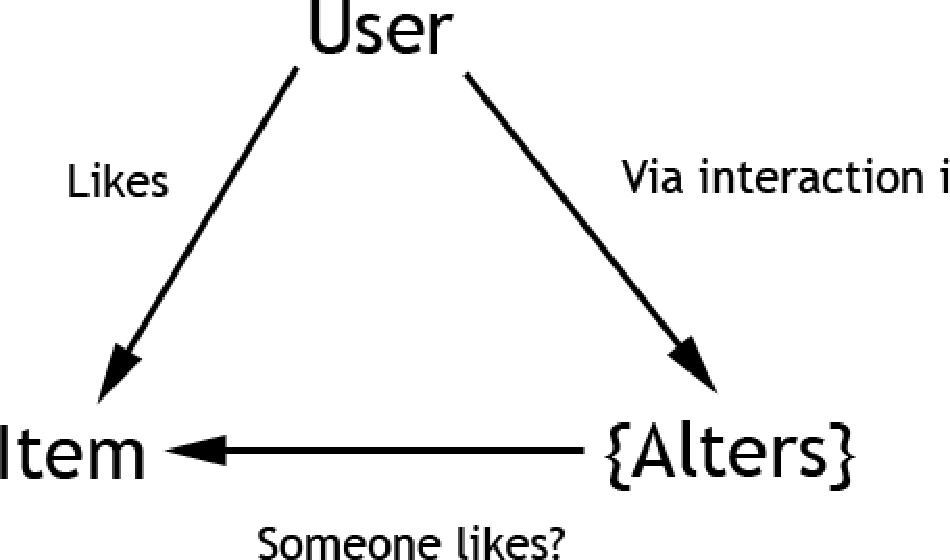
\includegraphics[scale=0.60]{imgs/alters.pdf}
		\caption{Alters paradigm. A user $u$ likes some item $v$, a $Relationship_{u,z}$ is defined via some affinity $i$ (in this example we use \emph{interactions}) uniquely defined
		for each affinity feature, to create our set of $alters_{u,v}$.}
	\end{center}
\end{figure}

\item An exposure limit where $Exposure_{u,v} = \displaystyle\sum_{z}^{N} (Friend_{u,z} \wedge Liked_{z,v})$ where this exposure can be 
limited by some $k$ with the condition $Exposure_{u,v} >= k$.

This exposure can be visualised in the figure below:

\begin{figure}[tbh!]
	\begin{center}
		\includegraphics[scale=0.65]{results/imageLiked.png}
		\caption{Here we see an example of a link $v$ posted to a friends wall, which has subsequently been liked by two friends $z$. This 
				 demonstrates an exposure of $2$ for $v$.}
	\end{center}
\end{figure}

\item A data-set $D$ comprised of $D = \{(u,v,x) \to y\}$ where $u \in U$, $v \in V$ and the binary response $y \in \{0,1\}$ 
where $0$ represents a dislike and $1$ represents a like. 
\end{itemize}

\section{Affinity Features}
\label{sec:features}

Given the vast amount of potential affinity features available on Facebook, we need to group our features into two 
distinct sets. Our two main headings will be \emph{user interactions} and \emph{user preferences}.

The individual components of these groups are displayed below:

\emph{User interactions}:
\begin{itemize}
\item \textbf{Interactions} : Posts, tags, likes, comments between users.
\item \textbf{Outgoing Messages} : Messages sent to other users.
\item \textbf{Incoming Messages} : Messages received from other users.
\end{itemize}

\emph{User preferences}:
\begin{itemize}
\item \textbf{Demographics} : Age, gender and location of a user.
\item \textbf{Favourites} : A users favourite preferences for activities, books, athletes, teams, movies, music, sports, television, people and interests.
\item \textbf{Groups} : All groups a user has joined.
\item \textbf{Pages} :  All pages a user has liked.
\end{itemize}

Each of these affinity features will be discussed in detail under their separate sections of this thesis.
During our analysis we will compare the predictiveness of each of these affinity features individually, as well as in combination.

\section{Previous Work}
\label{sec:pw}

Two general approaches to prediction in a social context are \emph{content-based filtering} (CBF) \cite{newsweeder} which exploits 
item features based on items a user has previously liked and  \emph{collaborative filtering} (CF) 
\cite{collab_filtering} which exploits the current users preferences as well as those of other users. 

Previous work defined the term \emph{social} CF (SCF) \cite{joseph} which augments traditional CF methods with additional social 
network information, the results of this previous work and analysis using live user trials came to the conclusion that the approach of SMB
provided the best results for this data set and as such will be used as a baseline.

These methods of CBF, CF and SCF result in a user gaining some similarity measure between other users, while the affinity features we 
explore during this thesis are based on explicit \emph{user interaction} and \emph{user preference} features and result in different 
models and predictions based on our feature selection.

\section{Training and Testing}
\label{sec:tt}

All evaluation is applied using $10$ fold cross validation wherein the data is partitioned into $10$ complementary subsets, $80\%$ of 
these subsets are used for training while the remaining $20\%$ are used for testing.

The training and testing process is repeated $10$ times for each set of fold data. These results are then averaged to produce our 
estimates and standard error. The benefit of this method over repeated sub-sampling is all data points are used for both training 
and validation.

\section{Classification Algorithms}
\label{sec:meth}

Each classification algorithm is passed the training data for each fold as outlined above. The classifier 
builds a model representation of the data and applies this model to the test set to classify each test item into either a dislike $0$ or 
a like $1$.

All affinity feature analysis carried out in this thesis will be performed on the following classification algorithms:

\subsection{Constant}
\label{sec:const}

The constant predictor returns a constant result irrespective of the affinity feature selected. Namely, this predictor returns dislike
regardless of the affinity feature represented by $X$. The most common result in our data set is dislike and hence this dislike 
predictor is displayed in all comparison analysis, tables and graphs.

\subsection{Social Match Box}
\label{sec:sr}

SMB is an extension of existing SCF techniques~\cite{lla,socinf} which constrain the latent space to enforce users 
who have similar preferences to maintain similar latent representations when they interact heavily.

SMB uses the social regularization method which incorporates user features to learn
similarities between users in the latent space which allows us to incorporate the social information of the Facebook data ~\cite{joseph}.

This objective component constrains users with a high similarity rating to have the same values in the latent feature space, which
models the assumption that users who are similar socially should also have similar preferences for items.

\subsection{Naive Bayes}
\label{sec:nb}

NB is a basic probabilistic classifier which involves applying Bayes' theorem using strong conditional independence 
assumptions between each feature in $X$. During training each element $i$ in $X$ is devised to contribute some 
evidence that this $x_i$ belongs to either a like or dislike classification, during testing the class with the highest probability 
when applied to the model is the classification predicted. 

With feature vector $f \in \mathbb{R}^F$ derived from $(x,y) \in D$, denoted as $f_{x,y}$. NB learns a conditional model of the form 
$p(C|F_1, \dots, F_n)$ over a dependent class variable $C$ conditioned on the feature variables $F_1, \dots, F_n$. Applying both Bayes' rule 
and conditional independence assumptions the model can be rewritten as $p(C|F_1, \dots, F_n) = p(C) \displaystyle\prod_{i=1}^n p(F_i|C)$.

Classification of our test vector is achieved by choosing the most probable class of either like ($1$) or dislike ($0$).
\\
$\mathrm{classify}(f_1,\dots,f_n) = \underset{c \in \{1,0\}}{\operatorname{argmax}} \ p(C=c) \displaystyle\prod_{i=1}^n p(F_i=f_i\vert C=c)$.

\subsection{Logistic Regression}
\label{sec:lr}

LR directly estimates parameters based on the training data assuming a parametric form of the distribution.
LR predicts the odds of a feature vector $X$ being either a like or a dislike by converting a dependent variable and 
one or more continuous independent variable(s) into probability odds.

The probability $p_i$ is modelled using a linear predictor function $l(i)$, the linear predictor function of a particular point $d$ 
is written as $l(i) = \beta_0 + \beta_1 x_{1,i} + \cdots + \beta_M x_{m,i}$, where each data point $d$ is associated with an explanatory 
feature vector $X$ and $\beta_0, \ldots, \beta_M$ are regression co-efficients indicating the relative effect of a particular 
explanatory variable $x_{m,i}$ on the prediction.

The probability of a particular outcome is linked to the linear prediction function, 
$\operatorname{logit}(\mathbb{E}[Y_i|x_{1,i},\ldots,x_{m,i}]) = \operatorname{logit}(p_i)=\ln\left(\frac{p_i}{1-p_i}\right) = \beta_0 + \beta_1 x_{1,i} + \cdots + \beta_M x_{m,i}$
Where the class of either dislike ($0$) or like ($1$) with the higher probability is the prediction made.

The LR implementation used during this thesis is \emph{LingPipe} \cite{lin}.

\subsection{Support Vector Machine}
\label{sec:svm}

SVM is a supervised learning machine based on a set of basis functions which help construct 
a separating hyperplane between data points. Training involves building the relevant hyperplanes which can then be used for testing. 
Each data point is classified as a like or dislike depending on which side of the hyperplane it falls.

With feature vector $f \in \mathbb{R}^F$ derived from $(x,y) \in D$, denoted as $f_{x,y}$. A linear SVM learns a weight vector $w \in \mathbb{R}^F$
such that $w^T f_{x,y} > 0$ indicates a like classification of $f_{x,y}$ and $w^T f_{x,y} \leq 0$ indicates a dislike classification.

The SVM implementation used during this thesis is \emph{SVMLibLinear} \cite{cjlin}.

\section{Evaluation Metrics}
\label{sec:notation}

When evaluating the success of each affinity feature at correctly classifying an item, the following metrics are used:

\begin{itemize}
\item A \emph{true positive} (TP) prediction refers to when the prediction correctly identifies the class as true. 
\item A \emph{false positive} (FP) occurs when the prediction is true, but the true class was false.
\item A \emph{false negative} (FN) occurs when the prediction is false but the actual class is true.
\end{itemize}

These definitions can be visualised using the table below:

\begin{table}[tbh!]
\centering
\begin{tabular}{r|l|l|l|}
\multicolumn{1}{r}{}
 &  \multicolumn{3}{c}{$y$} \\
 \cline{2-4}
& & \textbf{T} & \textbf{F} \\ 
\cline{2-4}
$\hat{y}$ & \textbf{T} & TP & FP \\
\cline{2-4}
& \textbf{F} & FN & TN \\
\cline{2-4}
\end{tabular}
\caption{Actual and prediction comparison table.}
	\label{tab:revpol}
\end{table}

Where $y$ represents the true class value $y \in \{0,1\} : actual$ and $\hat{y}$ represents the class prediction $\hat{y} \in \{0,1\} : prediction$.

Accuracy relates to the closeness to the true value. In the context of our results, the accuracy refers to the number of correct classifications 
divided by the size of the data set.

\[ \text{accuracy} = \frac{\text{number of correct classifications}}{\text{size of the test data set}}\]

Precision relates to the number of retrieved predictions which are relevant. In the context of our results, the precision refers to the number of TP predictions 
divided by the sum of the TP and FP predictions.

\[ \text{precision} = \frac{\text{number of TP}}{\text{number of TP + number of FP}}\]

Recall refers to the number of relevant predictions that are retrieved. In the context of our results, recall refers to the number of TP predictions 
divided by the sum of the TP and FN predictions.

\[ \text{recall} = \frac{\text{number of TP}}{\text{number of TP + number of FN}}\]

The f-score combines and balances both precision and recall and is interpreted as the weighted average of both precision and recall. 

\[ \text{f-score} = 2 \times \frac{\text{precision} \times \text{recall}}{\text{precision} + \text{recall}}\]

The main metric we use for analysis, tabulation and graphing in our results is accuracy.

%%% Local Variables: 
%%% mode: latex
%%% TeX-master: "thesis"
%%% End: 


\section{New Objective Functions for SCF}
\label{sec:NewObjFuns}
Having surveyed previous CF work, especially MF-based CF and SCF
methods, we now present the major conceptual contributions of the
paper.  However, before we get into details, we introduce a unified
matrix factorization framework for optimizing all MF objectives
evaluated in this paper, including newly proposed objectives to
address observed deficiencies of SCF MF methods as outlined in
Section~\ref{sec:Introduction}.

\subsection{A Composable Objective Framework}

%\subsubsection{Composable Objectives}

We take a composable approach to MF-based (S)CF, where an optimization
objective $\mathit{Obj}$ is composed of sums of one or more objective
components:
\begin{align}
\mathit{Obj} = \sum_i \lambda_i \mathit{Obj}_i
\end{align}
Because each objective may be weighted differently, a weighting term
$\lambda_i \in \R$ is included for each component.  In the current work,
we manually tuned each $\lambda_i$, except for the last $i$ in $\sum_i$,
which can be set as $\lambda_i = 1$ without loss of generality.

Most target predictions in this paper are binary ($\{0,1\}$),
therefore a sigmoidal transform $\sigma(o) = \frac{1}{1 + e^{-o}}$ of
a prediction $o \in \R$ may be used to squash it to the range $[0,
1]$.  Where the $\sigma$ transform may be optionally
included, this is written as $[\sigma]$.  While $\sigma$ transforms
are generally advocated for real-valued regressor outputs when used in
a classification setting, we note that our experiments showed little
variation in results whether including or omitting it, although
including it tended to slow the convergence of gradient optimization.
Nonetheless, where appropriate, we include the possibility of a
$\sigma$ transform since it may prove useful in other settings.

\subsection{Existing Objective Functions}

For completeness, we first cover a number of known objective
components that are used in the objectives evaluated and
extended in this paper.  A discussion of gradient optimization along
with all necessary derivatives for these objectives is provided in
Appendix~\ref{app:Derivatives}.

\subsubsection{Matchbox-style Matrix Factorization ($\Obj_\pmcf$)}

\label{sec:matchbox_def}

%As a first step towards addressing our first observed deficiency that
%%the six surveyed SCF MF methods of Section~\ref{sec:scf_original} do not
%exploit user or item features.  In extending these methods to support
%features, we must first identify
In Section~\ref{sec:mf}, we discussed an MF objective~\eqref{eq:basic_mf}
that \emph{did not} make use of user or item features.  
However, if we \emph{do} have user feature vector $\x$ 
and item feature vector $\y$, we can respectively
represent the latent projections of user and item as $(U \x)_{1 \ldots
K}$ and $(V \y)_{1 \ldots K}$ and hence use $\la U \x, V \y \ra = \x^T
U^T V \y$ as a measure of affinity between user $\x$ and item $\y$.
Substituting the feature-based $\x^T U^T V \y$ for the featureless 
$U_\x^T V_\y$ in~\eqref{eq:basic_mf}, we arrive at the form of the basic CF 
objective function used in \emph{Matchbox}~\cite{matchbox} --- although
Matchbox used Bayesian optimization methods, we can easily express
its objective in the following log likelihood form:
\begin{align}
\Obj_\pmcf & = \sum_{(\x,\y) \in D} \frac{1}{2} (R_{\x,\y} - [\sigma] \x^T U^T V \y)^2 \label{eq:matchbox_obj}
\end{align}
%It should be clear that if $\x$ and $\y$ are simply binary vectors
%of mutually exclusive user and item IDs, then this form reduces
%to~\eqref{eq:basic_mf}.  However, in general it permits general real-valued
%feature vectors for $\x$ and $\y$ and hence a feature-based MF approach to CF.

\subsubsection{Regularization of $U$, $V$, \& $\w$ ($\Obj_\ru, \Obj_\rv, \Obj_\w$)}

To help in generalization, it is important to regularize any free
matrix parameters $U$ and $V$ (e.g., from
Section~\ref{sec:matchbox_def}) or vector parameters $\w$ (e.g., from
Section~\ref{sec:cbf}) to prevent overfitting in the presence of
sparse data. This can be done with a simple $L_2$ regularizer that
models a spherical Gaussian prior of $0$ on the parameters.  This
regularization component can be specified for $U$, $V$, and $\w$
simply as follows:
\begin{align}
\Obj_\ru & = \frac{1}{2} \| U \|_\Fro^2 = \frac{1}{2} \tr(U^T U) \qquad
\Obj_\rv = \frac{1}{2} \tr(V^T V) \nonumber \\
\Obj_\rw & = \frac{1}{2} \| \w \|_2^2 = \frac{1}{2} \w^T \w \label{eq:reg}
\end{align}

\subsection{New Objective Functions}

\label{sec:newobjfun_defs}

Now we return to our observations concerning the deficiencies of
existing SCF MF methods as outlined in Section~\ref{sec:Introduction}
and propose new objective functions to address these issues.  
Gradient optimization for these new objectives and all necessary derivatives 
are covered in Appendix~\ref{app:Derivatives}.

\subsubsection{Feature Social Regularization ($\Obj_\rs$ \& $\Obj_\rss$)}
\label{sec:SocRec}

Our previous discussion of SCF methods in Section~\ref{sec:scf_original}
covered three different methods for \emph{social regularization} --- that is,
constraining users to be similar based on evidence from the social network.
However, none of these previous three SCF social regularization methods
exploited user features in the \emph{learning} process; more precisely 
$U_\x$ and $U_\z$ were regularized, but not the feature-based latent
spaces $U\x$ and $U\z$.  Hence if a gender difference in $\x$ and $\z$ was the
crucial factor to differentiating the latent spaces of each user, it \emph{could} 
be learned if we had a way of socially regularizing $U\x$ and $U\z$
directly.  To address this, we provide two variants of 
\emph{feature-based social regularization}.

The first new objective is an extension of simple 
\emph{social regularization}~\cite{lla,socinf} by incorporating user
features into that objective:
\begin{align}
\Obj_\rs = & \sum_{\x} \sum_{\z \in \mathit{friends}(\x)} \frac{1}{2} (S_{\x,\z} - \la U\x, U\z \ra)^2 \\
& = \sum_{\x} \sum_{\z \in \mathit{friends}(\x)} \frac{1}{2} (S_{\x,\z} - \x^T U^T U \z)^2 \nonumber 
\end{align}

%\subsubsection{Social Spectral Regularization ($\Obj_\rss$)}

Alternately, we could extend \emph{social spectral
regularization}~\cite{sr,rrmf} by incorporating user features into the
objective:
\begin{align}
\Obj_\rss = & \sum_{\x} \sum_{\z \in \mathit{friends}(\x)} \frac{1}{2} S^+_{\x,\z} \| U\x - U\z \|_2^2 \\
%& = \sum_{\x} \sum_{\z \in \mathit{friends}(\x)} \frac{1}{2} S^+_{\x,\z} \| U (\x - \z) \|_2^2 \nonumber \\
& = \sum_{\x} \sum_{\z \in \mathit{friends}(\x)} \frac{1}{2} S^+_{\x,\z} (\x - \z)^T U^T U (\x - \z) \nonumber
\end{align}

While we note these extensions are straightforward, they have
the simple property that they allow the system to learn the latent
user projection matrix $U$ \emph{as a function of user features}
in order to minimize the social regularization penalty.
Compared to non-socially regularized CF objectives, we will
demonstrate that both of these approaches are quite powerful in 
Section~\ref{sec:EmpResults}.

%\subfive Note: standard spectral regularization 
%assumes $S^+_{\x,\z} \in [0,1]$;
%however we may also want to try $S_{\x,\z}$ since a negative value
%actively encourages the latent spaces to oppose each other, which may
%be desired.

\subsubsection{Hybrid Information Diffusion + SCF ($\Obj_\phy$ )}

\label{sec:hybrid_scf}

One major weakness of MF methods is that they cannot model direct
joint features over user and items --- they must model user and item
features independently in order to compute the independent latent
projections $U\x$ and $U\z$.  Unfortunately, this prevents standard MF
objectives from modeling direct user-to-user information
diffusion~\cite{inf_diffusion} --- the 
unidirectional flow of links from one user to another.
This is problematic because if user $\x$ \emph{always} likes what $\z$
has posted or liked, then we would like to shortcut the latent
representation and simply learn to recommend user $\z$'s likes and posts 
to user $\x$.

We fix this deficit of MF by introducing another objective component
in addition to the standard MF objective, which serves as
a simple linear regressor for such information diffusion
observations.  The resulting hybrid objective component then becomes a
combination of latent MF and linear regression objectives.

For the linear regressor $\w^T \f_{\x,\y}$, we make use of the
\emph{same} weight vector $\w$ and feature vector $\f_{\x,\y}$
mentioned in Section~\ref{sec:cbf}; $\f_{\x,\y}$ is fully defined for
our empirical evaluation in Section~\ref{sec:dataset}.  As previously
noted, $\f_{\x,\y}$ includes
\emph{joint} user and item features from the social network, in
particular binary
\emph{information diffusion}~\cite{inf_diffusion} features
for \emph{each} friend $\z \in \mathit{friends}_\x$ indicating if $\z$
liked (or disliked) $\y$.  As a consequence, learning $\w$ allows the
linear regressor to predict in a personalized way for any user $\x$
whether they are likely to follow their friend $\z$'s preference for $\y$.

Formally, to define our hybrid information diffusion + SCF objective,
we combine the output of the linear regression prediction with the
Matchbox prediction, to get a hybrid objective component. The full
objective function for this hybrid model is then
\begin{align}
\Obj_\phy = \sum_{(\x,\y) \in D} \frac{1}{2} (R_{\x,\y} - [\sigma] \w^T \f_{\x,\y} - [\sigma] \x^T U^T V y)^2
\end{align}
While again we note that this simple hybrid MF + linear regression
objective is straightforward, the ability to use joint user and item
features to model information diffusion between users turns out to be 
extremely powerful in our later experiments.

\subsubsection{Co-preference Regularization ($\Obj_\rsc$)}
\label{sec:rsc}

A crucial aspect missing from other SCF methods is that while two
users may not be globally similar or opposite in their preferences,
there may be sub-areas of their interests which can be correlated to
each other.  For example, two friends may have similar interests
concerning technology news, but different interests concerning
political news.  \emph{Co-preference regularization} aims to learn
such selective co-preferences.  The motivation is to constrain users
$\x$ and $\z$ who have similar or opposing preferences to be similar
or opposite in the same latent latent space relevant to item $\y$.

We use $\la \cdot, \cdot \ra_{\bullet}$ to denote a re-weighted inner
product. The purpose of this inner product is to tailor the latent
space similarities or dissimilarities between users to specific sets
of items.  This addresses the issue detailed in the previous paragraph by
allowing users $\x$ and $\z$ to be similar or opposite in the same
latent latent space relevant only to item $\y$.

The objective component for \emph{Co-preference regularization} along
with its expanded form is
\begin{align}
\Obj_\rsc & = \sum_{(\x,\z,\y) \in C} \frac{1}{2} (P_{\x,\z,\y} - \la U\x, U\z \ra_{V\y})^2 \\
& = \sum_{(\x,\z,\y) \in C} \frac{1}{2} (P_{\x,\z,\y} - \x^T U^T \diag(V\y) U \z)^2 \nonumber
\end{align}
We might also define a \emph{social co-preference spectral
regularization} approach, but our experiments so far have not indicated
this works as well as the above objective.  

In contrast to social regularization
defined previously, co-preference regularization does not require knowledge
of friendships or user interactions to determine co-preferences and hence
can find correlations between users who are not friends --- this important
observation will indeed surface in our forthcoming experimental evaluation.

\begin{comment}
\subsubsection{Social Co-preference Spectral Regularization ($\Obj_\rscs$)}
This is the same as the social co-preference regularization above, except that it uses the spectral regularizer format for 
learning the co-preferences.

 We use $\| \cdot \|_{2,\bullet}$ to denote a re-weighted $L_2$ norm. The reweighing of this norm servers the same purpose as the re-weighted inner product in Section~\ref{sec:rsc}, it tailors the similarities or dissimilarities between users to specific sets of items. This allows users $\x$
and $\z$ to be similar or opposite in the same latent latent space
relevant only to item $\y$.  
 
 The objective component for
 social co-preference spectral regularization along with its expanded form is
 
\begin{align}
\Obj_\rscs & = \sum_{(\x,\z,\y) \in C} \frac{1}{2} P_{\x,\z,\y} \| U\x - U\z \|_{2,V\y}^2 \\
%& = \sum_{(\x,\z,\y) \in C} \frac{1}{2} P_{\x,\z,\y} \| U (\x - \z) \|_{2,V\y}^2 \nonumber \\
& = \sum_{(\x,\z,\y) \in C} \frac{1}{2} P_{\x,\z,\y} (\x - \z)^T U^T \diag(V\y) U (\x - \z) \nonumber 
\end{align}
\end{comment}


\section{Evaluation Framework}
\label{sec:Evaluation}
In this chapter we first discuss our Facebook Link Recommendation
(LinkR) application and then proceed to discuss how it can be
evaluated using general principles of evaluation used in the
machine learning and information retrieval fields.

\subsection{Facebook}

Facebook is a social networking service that is currently the largest
in the world. As of July 2011 it had more that 750 million active
users. Users in Facebook create a profile and establish ``friend''
connections between users to establish their social network. Each user
has a ``Wall'' where they and their friends can make posts to.  These
posts can be links, photos, status updates, etc.  Items that have been
posted by a user can be ``liked'', shared, or commented upon by other
users.  An example of a link post on a Wall that had been liked
by others was provided previously in Figure~\ref{fig:ex_link}.

%\begin{figure}[h]
%\centering
%\subfigure{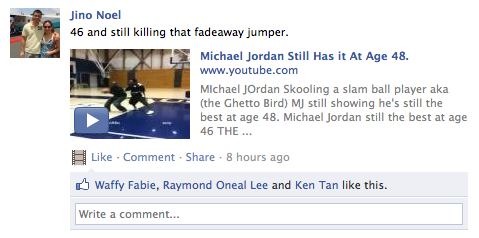
\includegraphics[scale=0.50]{img/posted-link.png}}
%\subfigure{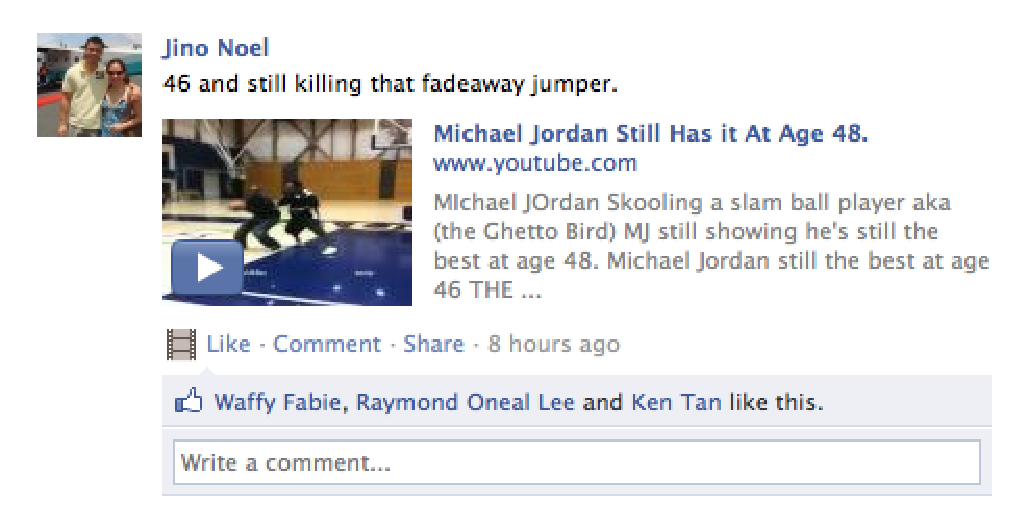
\includegraphics[scale=0.50]{img/posted-link.eps}}
%\caption{A link posted by the author that has been liked by three other users.}
%\end{figure}

This thesis seeks to find out how best to recommend links to
individual users such that there is a high likelihood that they will
``like'' their recommended links.  We do this by creating a
Facebook application (i.e., `Facebook ``App'') that recommends links
to users everyday, where the users may give their feedback on the
links indicating whether they \emph{liked} it or \emph{disliked} it.
We discuss this application in detail next.

\subsubsection{LinkR}

Facebook allows applications to be developed that can be installed by
their users.  As part of this thesis project, the LinkR Facebook
application was developed.\footnote{The main developer of the LinkR
Facebook App is Khoi-Nguyen Tran, a PhD student at the Australian
National University.  Khoi-Nguyen wrote the user interface and database
crawling code for LinkR.  All of the learning and recommendation
algorithms used by LinkR were written solely by the author for the
purpose of this thesis.}  The functionalities of the LinkR application
are as follows:
\begin{enumerate}
\item{Collect data that have been shared by users and their friends on Facebook.}
\item{Recommend (three) links to the users daily.}
\item{Collect feedback from the users on whether they liked or disliked the recommendations.}
\end{enumerate}

Figure~\ref{fig:linkr_app} shows the Facebook LinkR App as it appears
to users.
\begin{figure}[t!]
%\subfigure{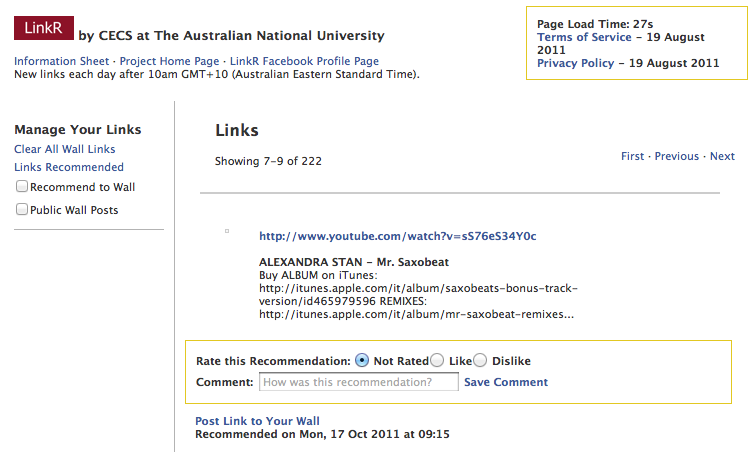
\includegraphics[scale=0.30]{img/linkr.png}}
\hspace{-2mm} \subfigure{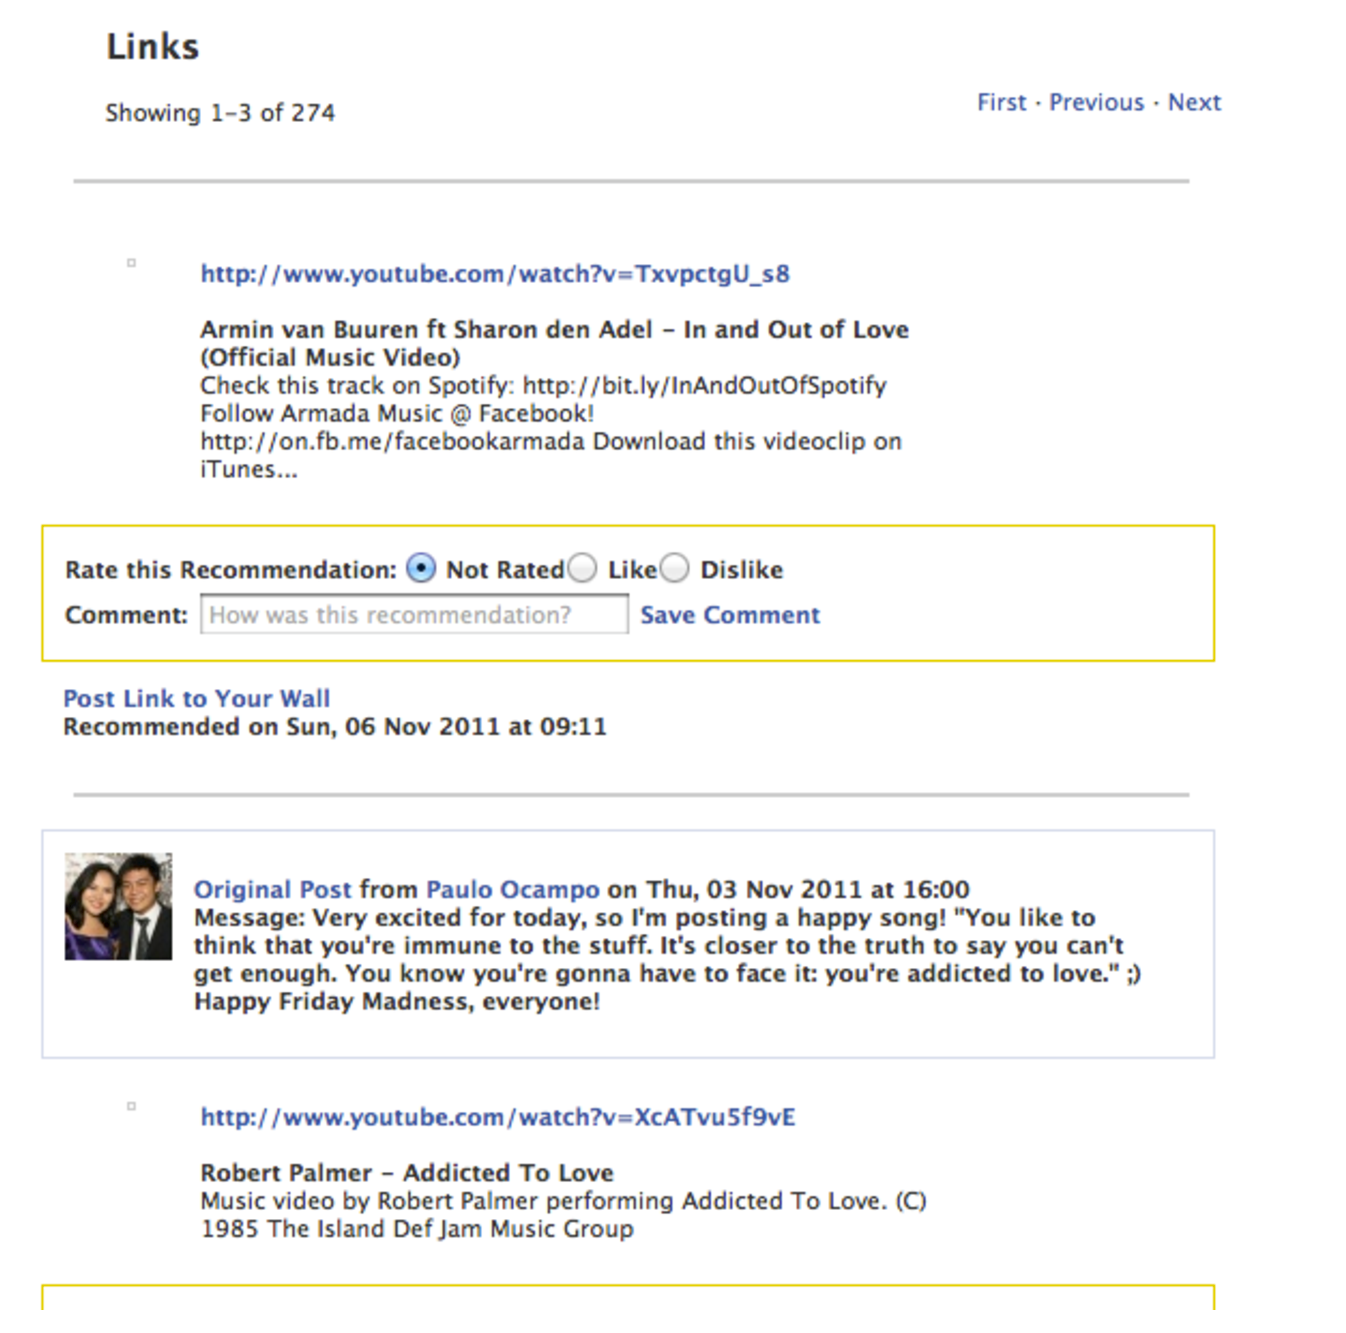
\includegraphics[scale=0.42]{img/linkr.eps}}
\caption{The Facebook LinkR App showing one of the recommendations
as it appears to users of the system.  Users have the option of liking
or disliking a recommendation as well as providing explicit feedback
commentary.}
\label{fig:linkr_app}
\end{figure}

\subsection{Dataset}

\label{sec:dataset}

Using the LinkR Facebook App developed for this project, we were able
to gather data on 34,860 users and 437,023 links.

\subsubsection{User Data}

Date that are collected and used for the user features are as follows:
\begin{itemize}
\item {Gender:} male or female
\item {Birthday:} year
\item {$\mathit{location}_\mathit{id}$:} an integer ID corresponding
to the user's specific present location (city and country)
\item {$\mathit{hometown}_\mathit{id}$:} an integer ID corresponding
to the user's specific home town (city and country)
\item {$F_{\x,\z} \in \{ 0, 1\}$:} indicator of whether 
users $\x$ and $\z$ are friends.
% Joseph: be specific here...
\item {$\mathit{Int}_{\x,\z} \in \mathbb{N}$:} interactions on
Facebook between users $\x$ and $\z$ as defined in Section~\ref{sec:notation}.
\end{itemize}

\subsubsection{Link Data}

Data that are used for the link features are:
\begin{itemize}
\item{$\mathit{id}$ of the user who posted the link.}
\item{$\mathit{id}$ of the user on whose wall the link was posted.}
\item{Text description of the link from the user who posted it.}
\item{Text link summary from the metatags on the target link webpage.}
\item{Number of times the link has been liked.}
\item{Number of times the link has been shared.}
\item{Number of comments posted on the link}.
\item {$F'_{\x,\y} \in \{0, 1\}$:} indicator of whether user $\x$ has liked item $\y$.
\end{itemize}
Additionally, links that have been recommended by the LinkR
application have the following extra features:
\begin{itemize}
\item{$\mathit{id}$'s of users who have clicked on the link url.}
\item{Optional ``Like'' or ``Dislike'' rating of the LinkR user on the link.}
\end{itemize}

\subsubsection{Interaction Data}
\label{sec:interactions}

The interactions between users that we count (equally weighted) to define
$\mathit{Int}_{\x,\z}$ are:

\begin{enumerate}
\item{Being friends.}
\item{Posting an item (link, photo, video, photo, or message) on a user's wall.}
\item{Liking an item (link, photo, video, photo, or message) on a user's wall.}
\item{Commenting on an item (link, photo, video, photo, or message) on a user's wall.}
\item{Being tagged together in the same photo.}
\item{Being tagged together in the same video.}
\item{Two users tagging themselves as attending the same school.}
\item{Two users tagging themselves as attending the same class in school.}
\item{Two users tagging themselves as playing sports together.}
\item{Two users tagging themselves as working together for the same company.}
\item{Two users tagging themselves as working together on the same project for the same company.}
\end{enumerate}

\subsubsection{Live Online Recommendation Trials}

For the recommendations made to the LinkR application users, we select
only links posted in the most recent two weeks that the user has not
liked. We use only the links from the last two weeks since an informal
user study has indicated a preference for recent links.  Furthermore,
older links have a greater chance of being outdated and are also
likely to represent broken links that are not working anymore. We have
settled on recommending three links per day to the LinkR users and
according to the survey done at the end of the first trial, three
links per day seems to be the generally preferred number of
daily recommendations.

For the live trials, Facebook users who installed the LinkR
application were \emph{randomly assigned one of four algorithms in
each of the two trials}. Users were not informed which algorithm was
assigned to them to remove any bias. We distinguish our recommended
links into two major classes, links that were posted by the LinkR
user's friends and links that were posted by users other than the
LinkR user's friends. The LinkR users were encouraged to rate the
links that were recommended to them, and even provide feedback
comments on the specific links. In turn these ratings became part of
the training data for the recommendation algorithms, and thus were used
to improve the performance of the algorithms over time. Based on the
user feedback, we filtered out non-English links and links without any
descriptions from the recommendations to prevent user annoyance.

At the end of the first trial, we conducted a user survey with the
LinkR users to find out how satisfied they were with the
recommendations they were getting.
 

\section{Empirical Results}
\label{sec:EmpResults}
In this section we discuss the algorithms evaluated in our two online
trials\footnote{All code used in these experiments is available at
\url{http://code.google.com/p/social-recommendation/}.  The conditions
of our ethics approval \#2011/142 from the Australian National
University for conducting human trials on Facebook require our
privacy policy
(\url{http://dmm.anu.edu.au/linkr/website/pp.php}) to
prohibit public sharing of data collected during these experiments.}
and additional analysis regarding trends and patterns in our social
recommendation setting.

\subsection{First Trial}

In our first trial, our objective was to evaluate four CF and SCF
approaches to establish which was the most promising direction for
SCF extension:
\begin{enumerate}
\item {\bf $k$-Nearest Neighbor (KNN)}: See Section~\ref{sec:nn}.
\item {\bf Support Vector Machines (SVM)}: See Section~\ref{sec:cbf}.
\item {\bf Matchbox (Mbox)}: simple Matchbox CF %Optimization of the $L_2$ regularized Matchbox objective:
$$\Obj_\pmcf + \lambda \Obj_\ru + \lambda \Obj_\rv$$
\item {\bf Social Matchbox (Soc. Mbox)}: %Optimization of the 
%$L_2$ and 
feature-based \emph{socially regularized} Matchbox SCF
$$\Obj_\pmcf + \lambda_\rs \Obj_\rs + \lambda \Obj_\ru + \lambda \Obj_\rv$$
\end{enumerate}
KNN and MBox may be viewed as pure CF methods.  As discussed previously,
both SVM and Soc. Mbox may be viewed as SCF methods
and were both optimized via gradient descent as outlined
in Appendix~\ref{app:Derivatives}.  

The first live user trial was run from August 25, 2011 to October 13, 2011 
with 108 users and yielded 2,493 combined like and 
dislike ratings of recommended
links over the 49 day period.  Algorithms were assigned randomly to the
users with assignment counts shown in Table~\ref{tab:Assigned1} (left).

%%%%%%%%%%%%%%%%%%%%%%%%%%%%%%%%%%%%%%%%%%%%%%%%%%%%%%%%%%
\begin{table}[t!]
\centering
\begin{minipage}{1.5in}
\begin{tabular}{| l | c |}
\hline
{\bf Algorithm} & {\bf Users} \\
\hline
Soc. Mbox & 26\\
Mbox  & 26 \\
SVM & 28 \\
KNN & 28 \\
\hline
\end{tabular}
  \end{minipage}
  \begin{minipage}{1.3in}
\begin{tabular}{| l | c |}
\hline
{\bf Algorithm} & {\bf Users} \\
\hline
Soc. Mbox & 26\\
Spec. Mbox  & 25 \\
Spec. CP & 27 \\
Soc. Hybrid & 25 \\
\hline
\end{tabular}
  \end{minipage}
\caption{Number of users assigned per algorithm in the first trial (left)
and second trial (right).}
\label{tab:Assigned1}
\end{table}
%%%%%%%%%%%%%%%%%%%%%%%%%%%%%%%%%%%%%%%%%%%%%%%%%%%%%%%%%%

As shown in Figure~\ref{fig:OnlineResult1}, Soc. Mbox was the
best performing algorithm in the first trial and in fact was the only
algorithm to receive more like ratings than dislike ratings. 
This suggests that using social regularization in conjunction with
MF-based CF does indeed provide more useful information than simple
MBox without social regularization.  We also note a
significant drop in performance between recommending friend links and
recommending non-friend links, indicating that users had a bias to
like links recommended by friends more (importantly, we note that
users could see the names and comments of friends whose links were recommended).
%%%%%%%%%%%%%%%%%%%%%%%%%%%%%%%%%%%%%%%%%%%%%%%%%%%%%%%%%%
\begin{figure*}[t!]
\centering
\subfigure{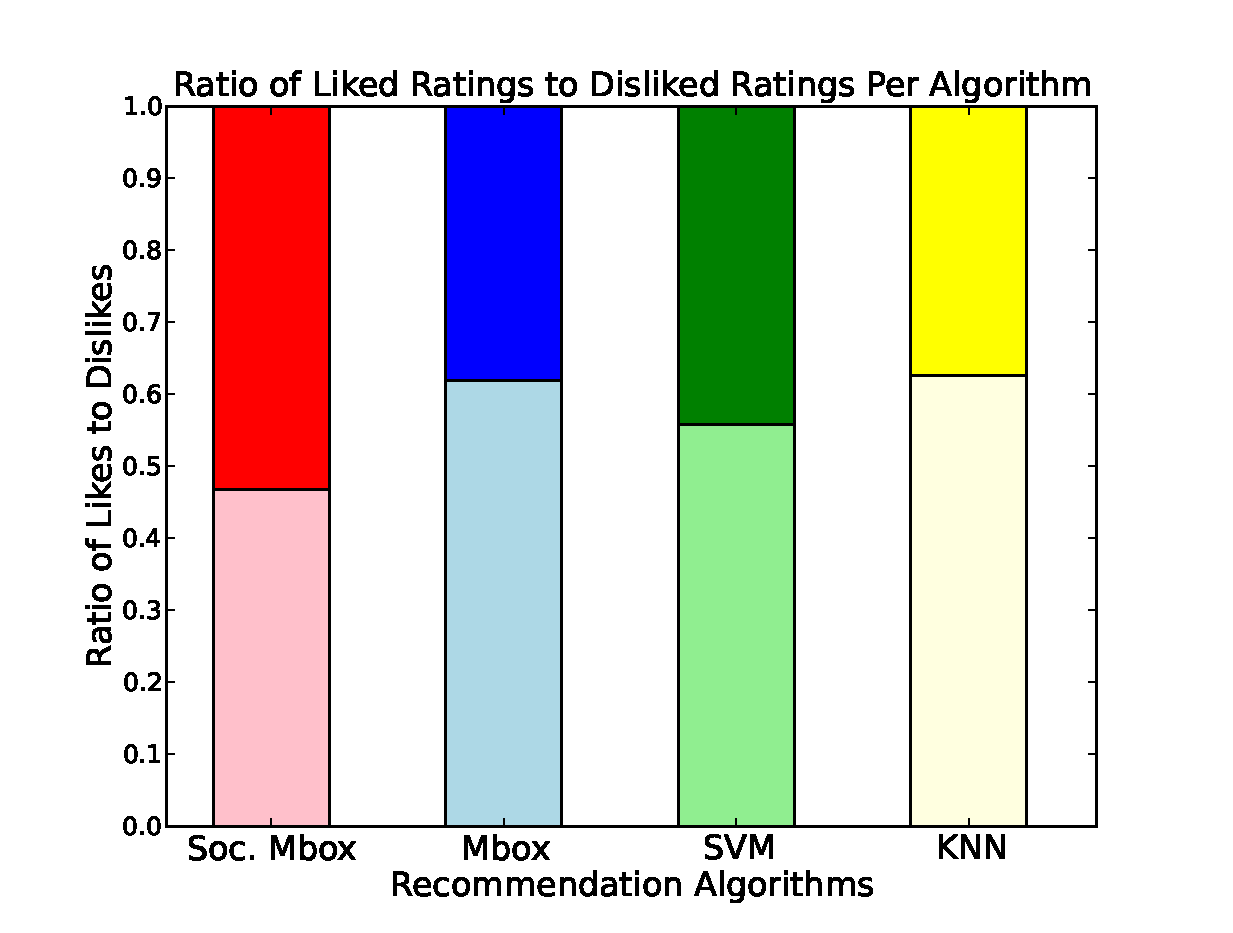
\includegraphics[scale=0.28]{img/live-likes1.eps}}
\subfigure{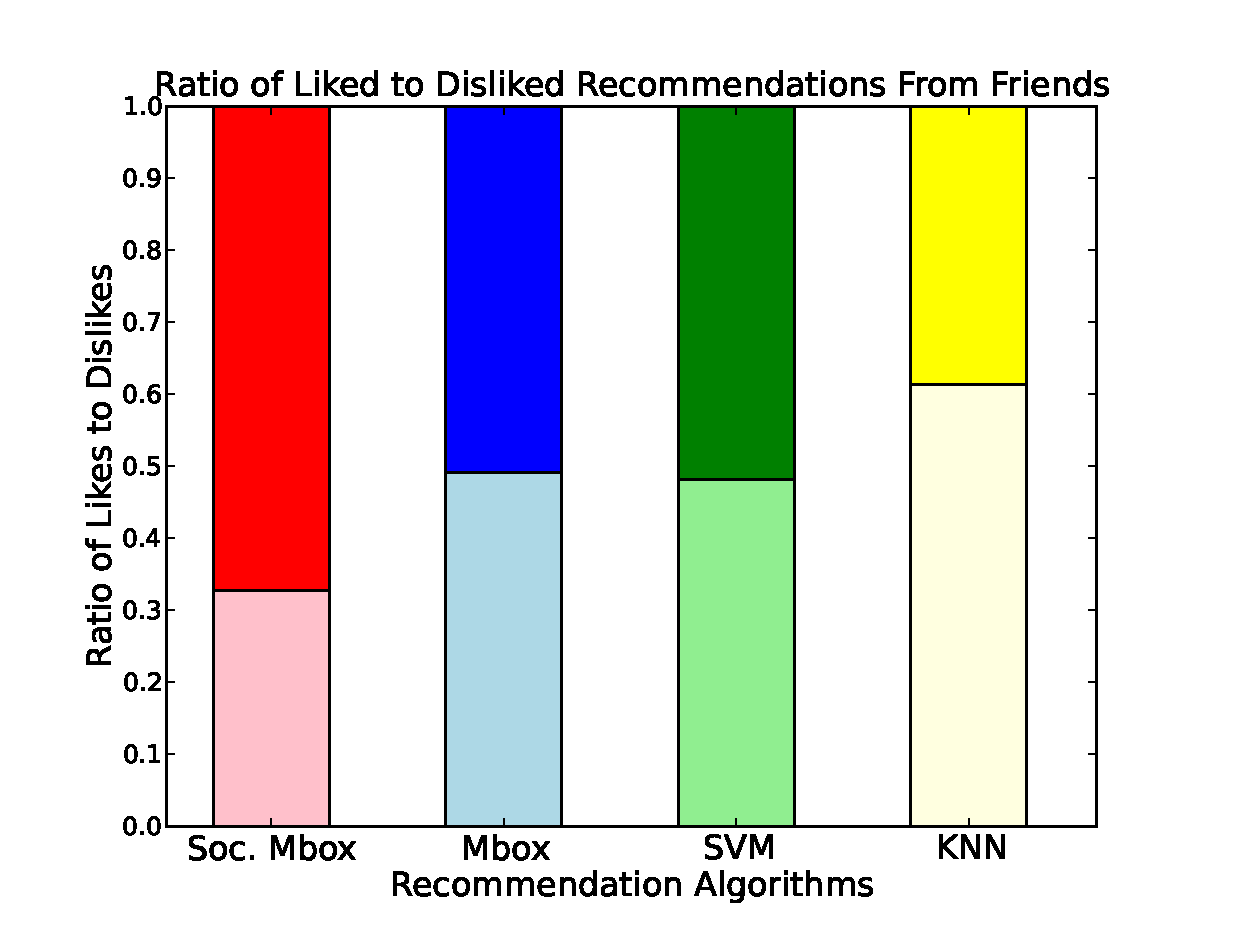
\includegraphics[scale=0.28]{img/live-friend-likes1.eps}}
\subfigure{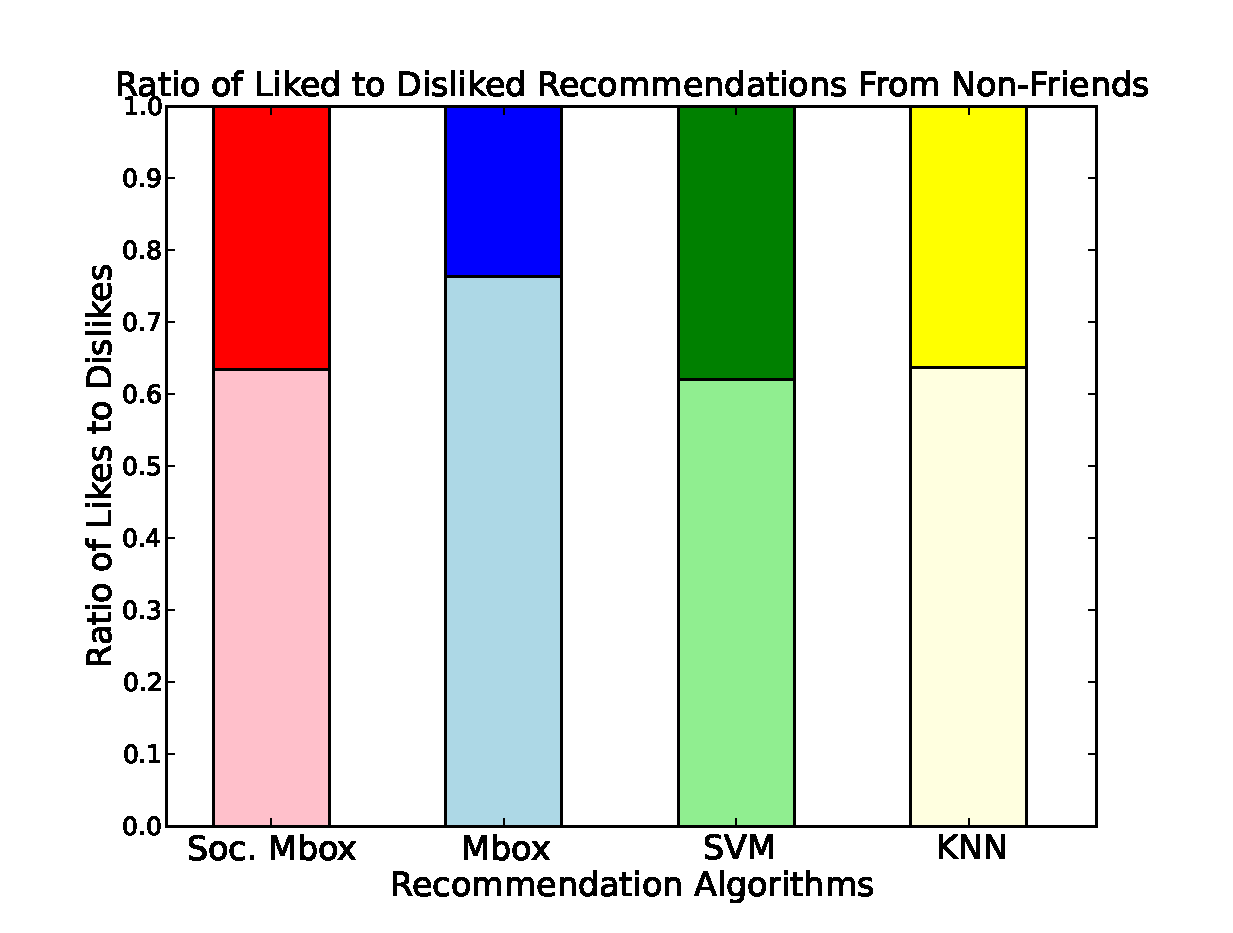
\includegraphics[scale=0.28]{img/live-nonfriend-likes1.eps}}
%\subfigure{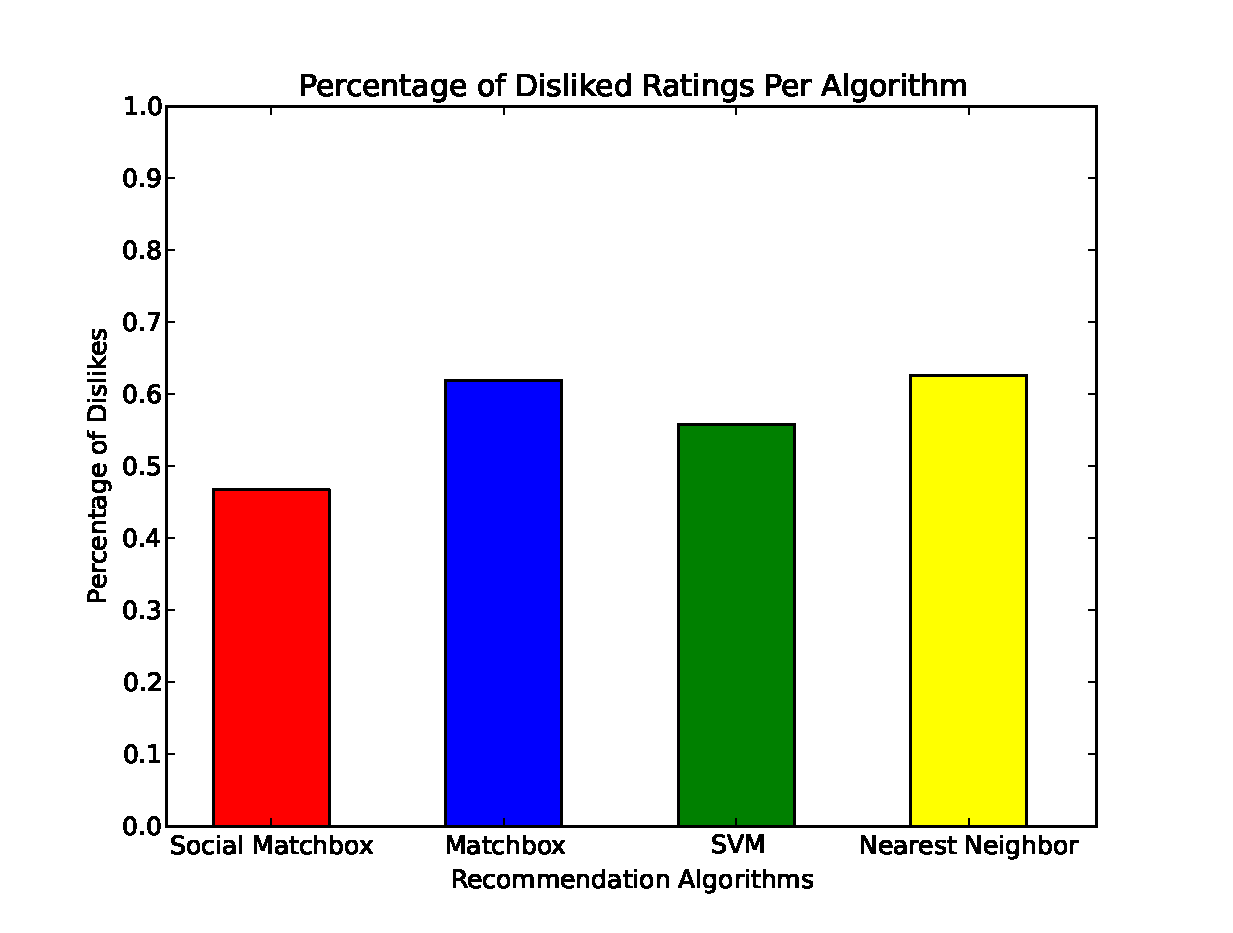
\includegraphics[scale=0.35]{img/live-dislikes1.eps}}
\caption{Stacked bar graphs of online results for the first 
user trial.  The fraction of likes is displayed above 
the fraction of dislikes.  (left) all links, (center) friend links,
(right) non-friend links.  The 95\% confidence interval on all 
results is $< \pm 0.02$ so all differences are signficant
except for MBox and SVM in the center and the virtual tie
between three algorithms on the right.}
\label{fig:OnlineResult1}
\end{figure*}
%%%%%%%%%%%%%%%%%%%%%%%%%%%%%%%%%%%%%%%%%%%%%%%%%%%%%%%%%%

%%%%%%%%%%%%%%%%%%%%%%%%%%%%%%%%%%%%%%%%%%%%%%%%%%%%%%%%%%
%%%%%%%%%%%%%%%%%%%%%%%%%%%%%%%%%%%%%%%%%%%%%%%%%%%%%%%%%%

\subsection{Second Trial} 

For the second online trial, we again chose four algorithms to
randomly assign to the LinkR application users.  Social Matchbox
was included again as a baseline since it was the best performing
algorithm in the first trial.  The remaining three algorithms
were all relatively orthogonal extensions (or variants) of Social Matchbox
based on the \emph{three novel objective functions} defined in 
Section~\ref{sec:newobjfun_defs}:
\begin{itemize}
\item {\bf Social Matchbox (Soc. Mbox)} : unchanged.
\item {\bf Spectral Matchbox (Spec. Mbox)}: 
$$\Obj_\pmcf + \lambda_\rss \Obj_\rss + \lambda \Obj_\ru + \lambda \Obj_\rv$$
%Matchbox MF + Social Spectral Regularization + L2 $U$ Regularization + L2 $V$ Regularization
\item {\bf Social Hybrid (Soc. Hybrid)}: 
$$\Obj_\pmcf + \lambda_\rs \Obj_\rs + \lambda_\phy \Obj_\phy + \lambda \Obj_\ru + \lambda \Obj_\rv$$
%Hybrid + Social Regularization + L2 $U$ Regularization + L2 $V$ Regularization + L2 $\w$ Regularization
\item {\bf Spectral Co-preference (Spec. CP)}: 
$$\Obj_\pmcf + \lambda_\rscs \Obj_\rscs + \lambda \Obj_\ru + \lambda \Obj_\rv$$
%Matchbox MF + Social Co-preference Spectral Regularization + L2 $U$ Regularization + L2 $V$ Regularization
\end{itemize}
All objectives are optimized via gradient descent as outlined
in Appendix~\ref{app:Derivatives}.  

The second trial with the above algorithms ran from October 13, 2011
to November 5, 2011 with 103 users and yielded 1,435 like/dislike
ratings of recommended links over the 24 day period; on the start of
the second trial, users were notified that they would be randomly
assigned to new algorithms and encouraged to re-engage with the LinkR
App if they had not been using it.  The distribution of the algorithms
to the users is shown in Table~\ref{tab:Assigned1} (right).

%%%%%%%%%%%%%%%%%%%%%%%%%%%%%%%%%%%%%%%%%%%%%%%%%%%%%%%%%%%%%%%%%%%%%%%%%
\begin{figure*}[t!]
\centering
\subfigure{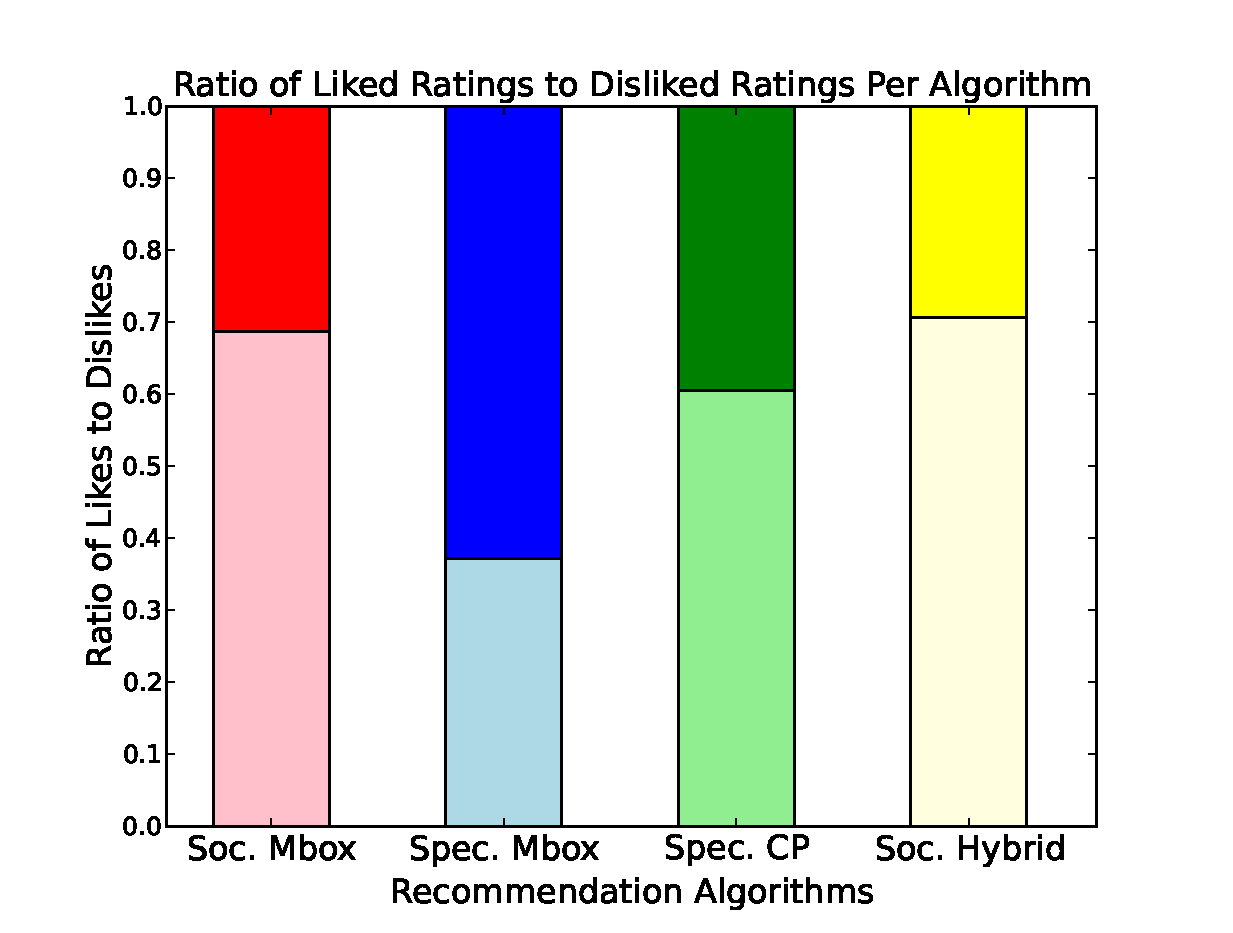
\includegraphics[scale=0.28]{img/live-likes2.eps}}
\subfigure{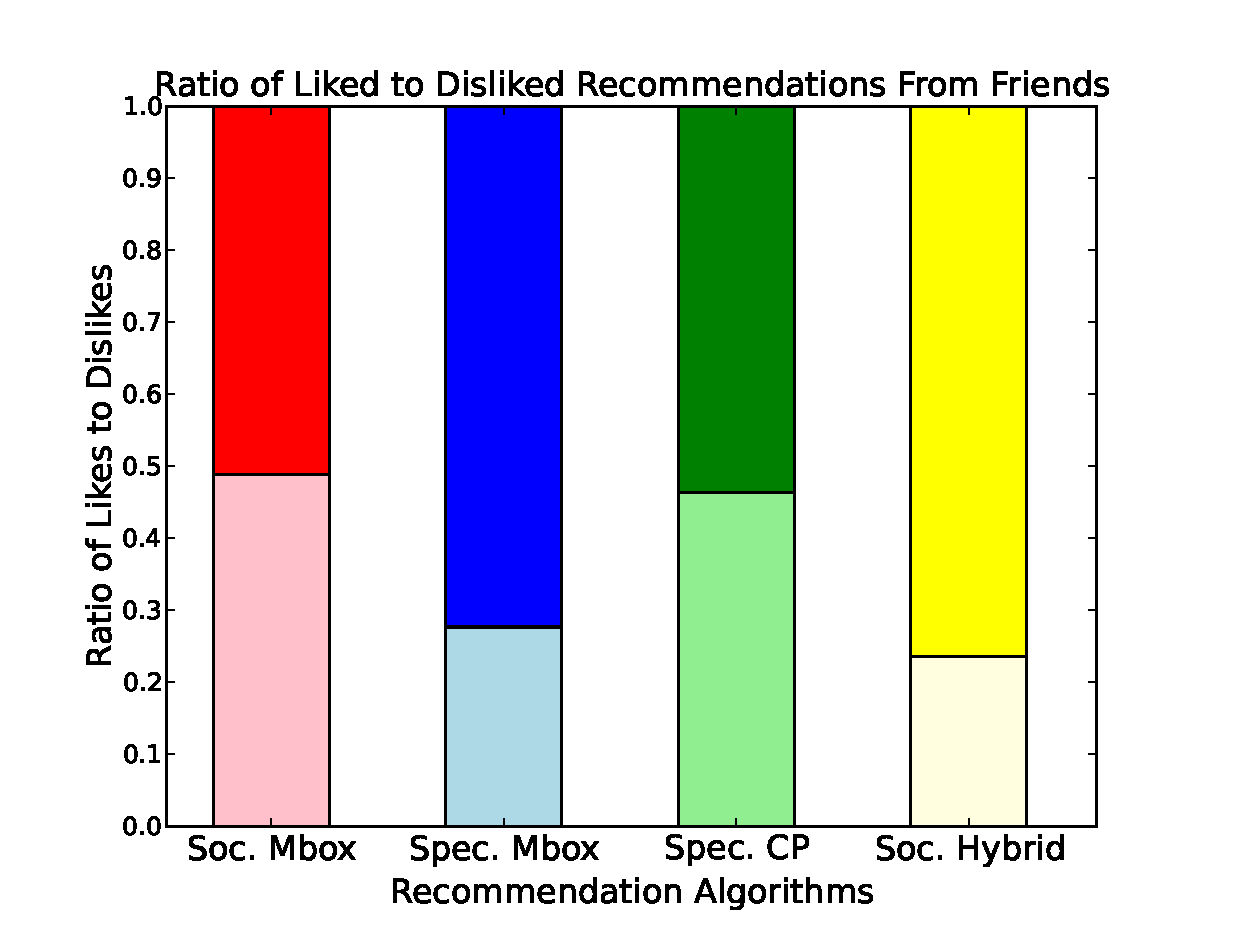
\includegraphics[scale=0.28]{img/live-friend-likes2.eps}}
\subfigure{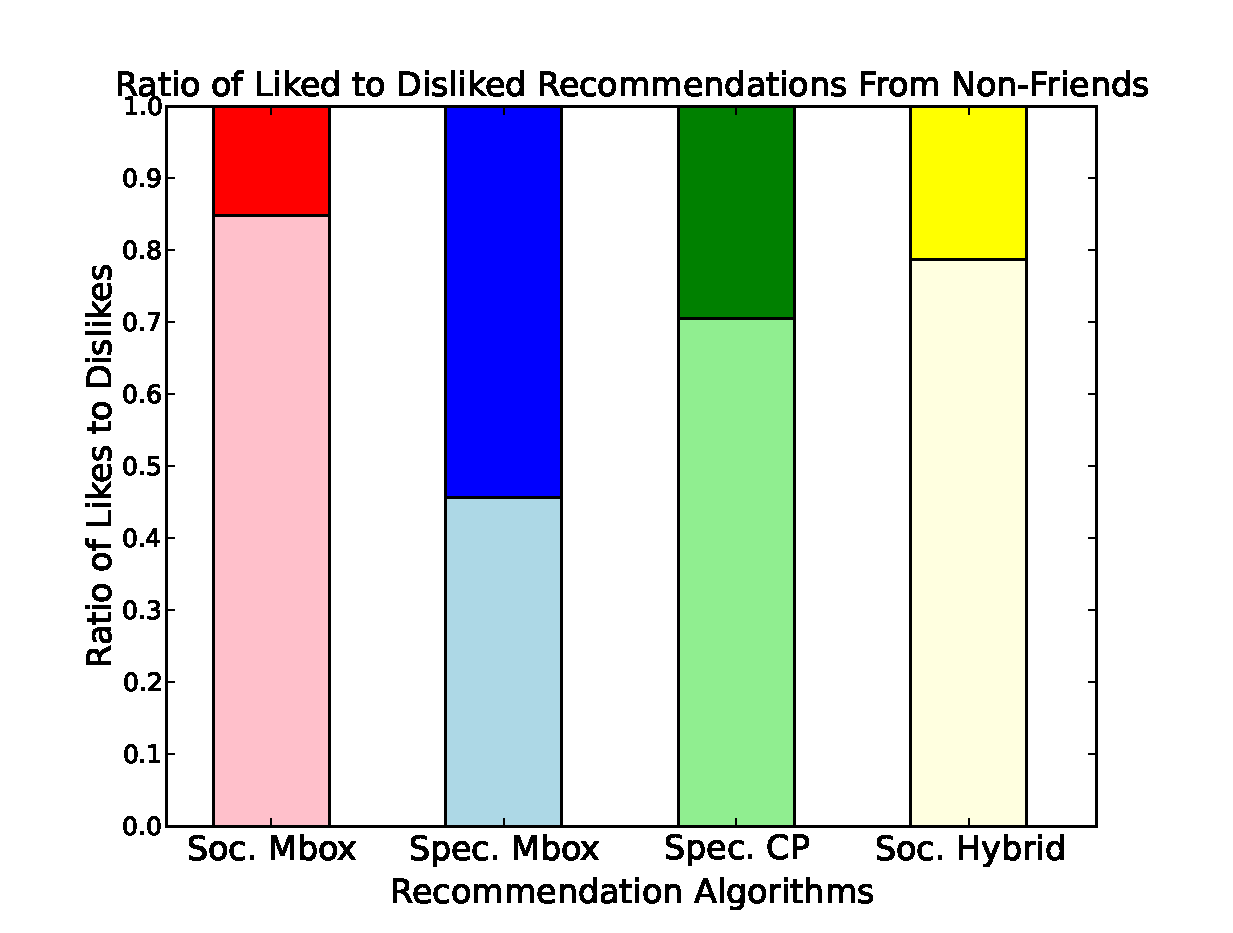
\includegraphics[scale=0.28]{img/live-nonfriend-likes2.eps}}
\caption{Stacked bar graphs of online results for the second
user trial.  The fraction of likes is displayed above 
the fraction of dislikes.  (left) all links, (center) friend links,
(right) non-friend links. The 95\% confidence interval on all 
results is $< \pm 0.026$ so all differences except Spec. Mbox
and Soc. Hybrid in the center graph are significant. }
\label{fig:online2}
\end{figure*}
%%%%%%%%%%%%%%%%%%%%%%%%%%%%%%%%%%%%%%%%%%%%%%%%%%%%%%%%%%%%%%%%%%%%%%%%%

Results for the second trial are 
shown in Figure~\ref{fig:online2}, following are the key observations:
\begin{itemize}
\item Soc. MBox did not perform as well in the second trial as it had
in the first trial.  One key difference in the second trial is that
all of the first trial data was available for training and thus
Soc. MBox may have been more difficult to optimize given this larger 
quantity of data (not available in the first trial).
\item Spec. Mbox clearly performed the best in the second trial 
and this suggests that spectral social 
regularization is likely a better method of regularization 
than the original social regularization variant.
\item Soc. Hybrid does an excellent job of capturing information diffusion
in the social network and hence performs best on recommending friend
links and most poorly on non-friend links (where there is no direct
user-to-user information diffusion).  Soc. Hybrid slightly outperforms
Spec. MBox, but not statistically significantly given the more limited
data in the second trial.  Nonetheless, 
Soc. Hybrid clearly outperform its Soc. MBox variant that lacks 
information diffusion features.
\item Spec. CP leads to a statistically significant improvement
on recommending non-friend links over Soc. MBox and Soc. Hybrid,
which perform poorly on recommending non-friend links.  Clearly then
Spec. CP is benefitting somewhat in learning from copreferences
since it can socially regularize across two users that are \emph{not}
friends.
\end{itemize}

%%%%%%%%%%%%%%%%%%%%%%%%%%%%%%%%%%%%%%%%%%%%%%%%%%%%%%%%%%
%%%%%%%%%%%%%%%%%%%%%%%%%%%%%%%%%%%%%%%%%%%%%%%%%%%%%%%%%%

\subsection{User Behavior Analysis}

\label{sec:behavior}

Here we briefly analyze user behavior during both trials of the Facebook
LinkR App that can be helpful in building future SCF systems.

\subsubsection{Click evidence}

In Figure~\ref{fig:click_evidence}, we observe the ratings of links
that users clicked on.  The most important thing we notice in 
Figure~\ref{fig:click_evidence} (left) is that even though users
clicked on a link, they were highly likely to rate it as a dislike.

One might hypothesize that perhaps users clicked on links more often with
no description to find out what they were and most often disliked them ---
this might explain the high number of dislikes for clicked links.  However,
examining both 
Figure~\ref{fig:click_evidence} (center) and 
Figure~\ref{fig:click_evidence} (right)
for non-friend links, we observe that whether a description was present
had very little impact on whether a link was liked or not, so we cannot
infer that all the disliked links were simply the ones lacking a description.

Then the insight from this analysis is extremely important 
for SCF recommendation design because it states that click data is a very
weak indicator of likes and explicit feedback should be used if at all
possible.

%%%%%%%%%%%%%%%%%%%%%%%%%%%%%%%%%%%%%%%%%%%%%%%%%%%%%%%%%%
\begin{figure*}[t!]
\centering
\subfigure{\includegraphics[scale=0.28]{img/clickedLikes.eps}}
\subfigure{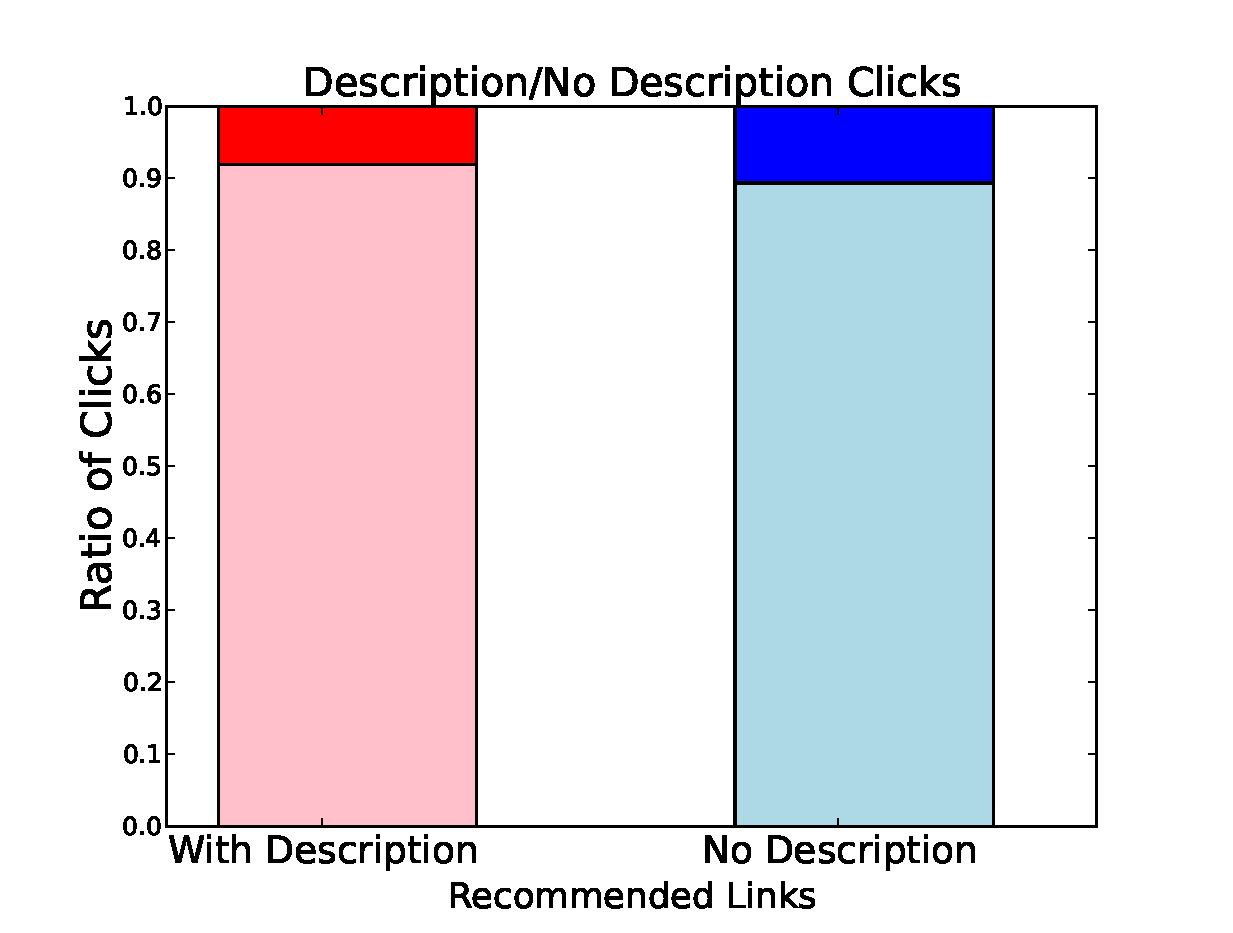
\includegraphics[scale=0.28]{img/descriptionClicked.eps}}
\subfigure{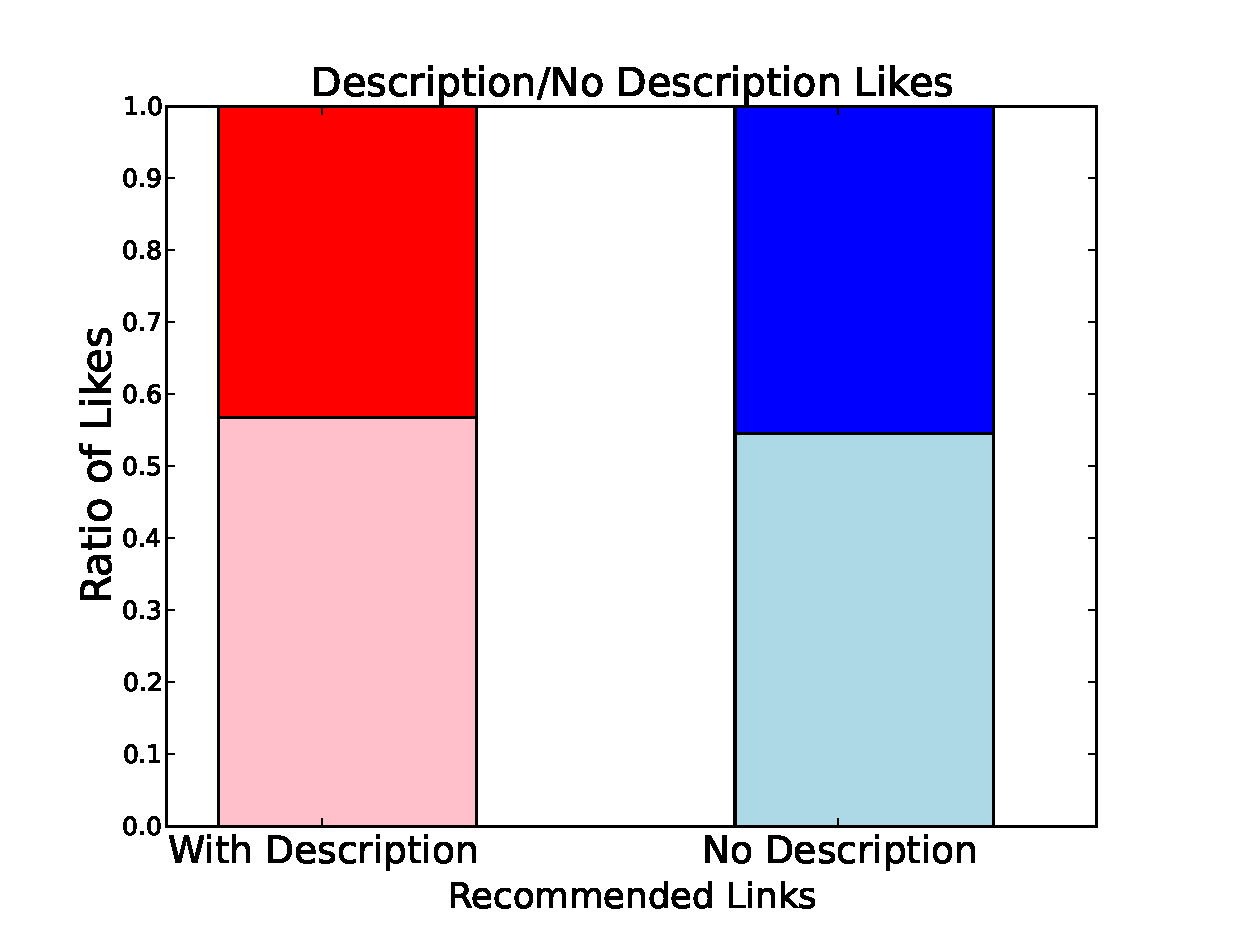
\includegraphics[scale=0.28]{img/descriptionLiked.eps}}
\caption{Stacked bar graphs of online results for the first 
user trial.  The fraction of likes (or clicks) is displayed above 
the fraction of dislikes (or non-clicks) -- and above the fraction of not-rated
links for the left-most figure.  
(left) ratings for clicked links, (center) click rates if
text description not present, 
(right) percentage liked if click description not present.}
\label{fig:click_evidence}
\end{figure*}
%%%%%%%%%%%%%%%%%%%%%%%%%%%%%%%%%%%%%%%%%%%%%%%%%%%%%%%%%%

\subsubsection{Impact of Popularity}

In Figure~\ref{fig:popularity} we analyze the impact of global link
popularity (in terms of total shares on Facebook) 
on how much Facebook LinkR App users liked a link.
The trend is clear for both friend (left) and non-friend (right)
links: users tend to like the most popular (top quartile) 
links the least, or at least as much as the least popular (bottom quartile)
links.  In general users tended to prefer links that were somewhat
popular (second highest quartile).  From this we can infer that
link popularity should not be used too heavily in determining link
recommendations since clearly the most popular links are not liked
the most on average.

%%%%%%%%%%%%%%%%%%%%%%%%%%%%%%%%%%%%%%%%%%%%%%%%%%%%%%%%%%
\begin{figure*}[t!]
\centering
\subfigure{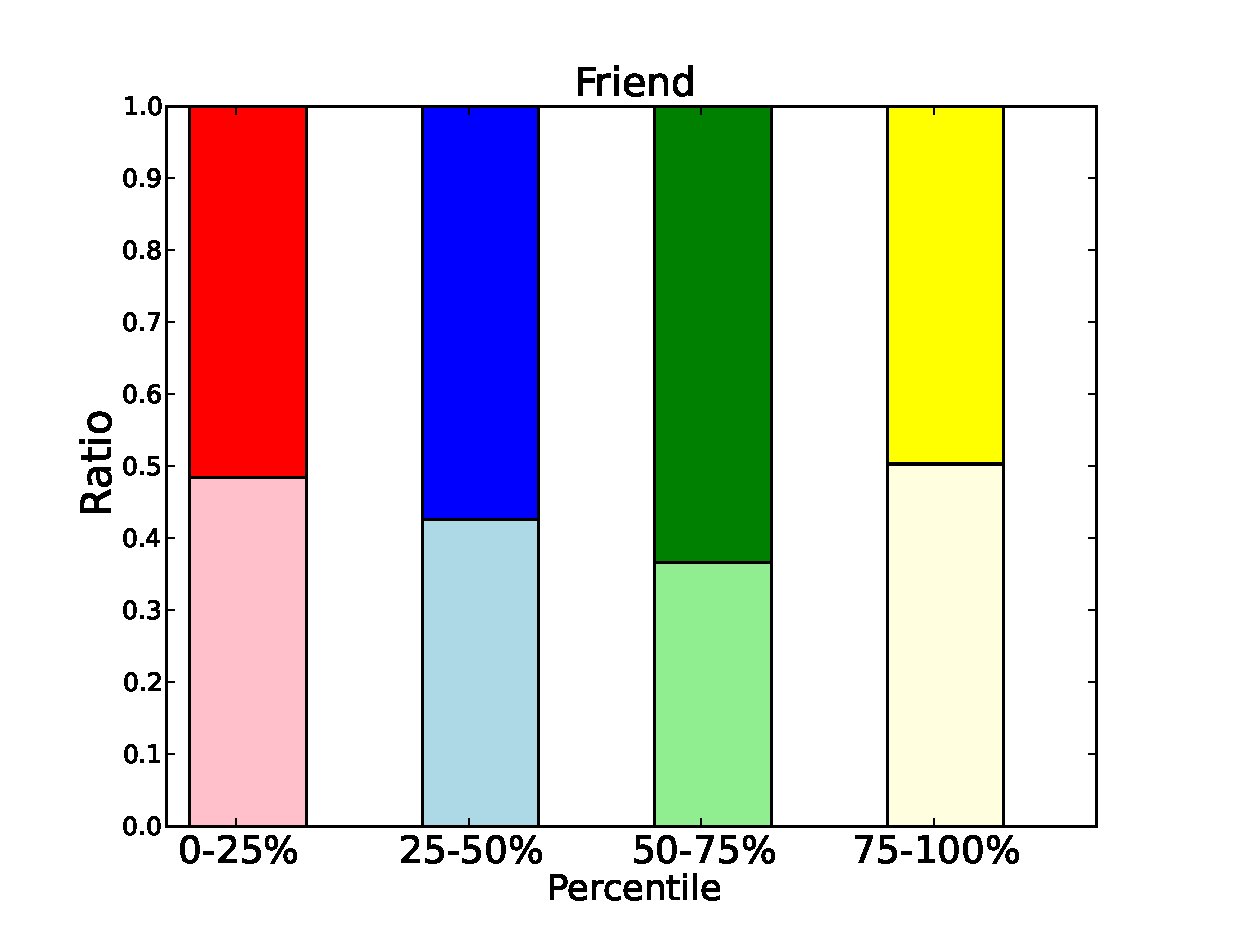
\includegraphics[scale=0.28]{img/percentileFriend.eps}}
\subfigure{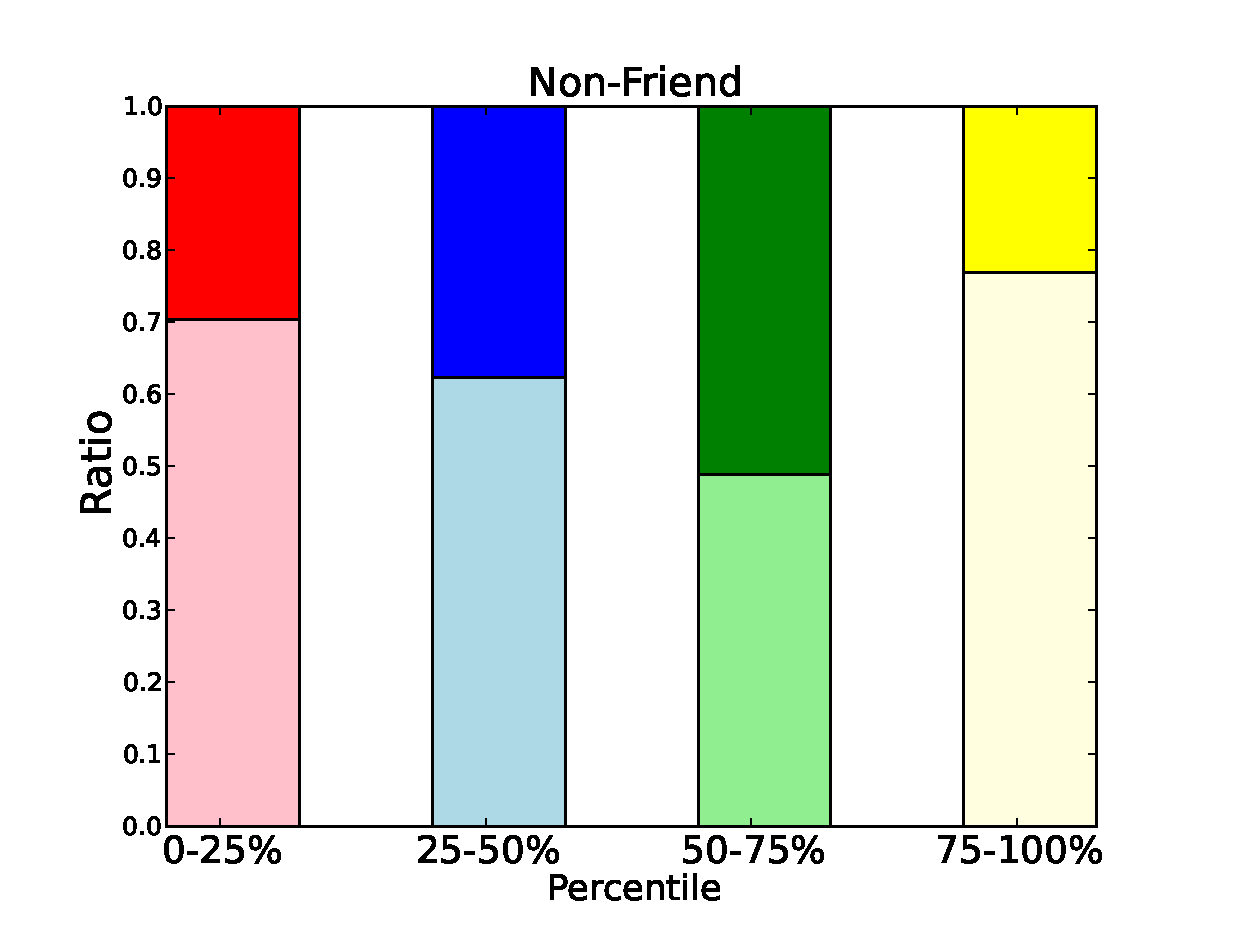
\includegraphics[scale=0.28]{img/percentileNon-Friend.eps}}
\caption{Stacked bar graphs of online results for the first 
user trial.  The fraction of likes is displayed above the fraction of
dislikes.  Shown are the ratings vs. quartile of popularity for (left)
friend and (right) non-friend links.}
\label{fig:popularity}
\end{figure*}
%%%%%%%%%%%%%%%%%%%%%%%%%%%%%%%%%%%%%%%%%%%%%%%%%%%%%%%%%%



\section{Conclusions}
\label{sec:Conclusions}
% This is rough, needs editing.

%\subsection{Summary}

In this paper, we evaluated existing algorithms and proposed new
algorithms for social collaborative filtering via the task of link
recommendation on Facebook.  Importantly, we outlined three main
deficiencies in existing social collaborative filtering (SCF) matrix
factorization (MF) techniques and proposed novel objective functions that 
learns user similarity from features using social spectral regularization,
models direct user-user information diffusion by extending Matchbox~\cite{matchbox}
and models restricted common interests with social co-preference regularization.

Having evaluated existing baselines variants and then
evaluating these new algorithms in Section~\ref{sec:EmpResults} in
live online user trials with over 100 Facebook App users and data for
over 30,000 unique Facebook users
This paper represents one concrete step forward in SCF
algorithms based on top-performing MF methods and their ability to
fully exploit the breadth of information available on social networks.

%% move these statements to end of INTRO
%\begin{itemize}
%\item[(a)] {\bf Non-feature-based user similarity:} 
%We extended existing social regularization and \emph{social spectral regularization} methods to incorporate \emph{user features} to learn user-user similarities in the latent space.
%\item[(b)] {\bf Model direct user-user information diffusion:} 
%We defined a new hybrid SCF method where we \emph{combined} the \emph{collaborative filtering (CF) matrix factorization (MF) objective} used by Matchbox~\cite{matchbox} with a \emph{linear content-based filtering (CBF) objective} used to model direct user-user information diffusion in the social network.
%\item[(c)] {\bf Restricted common interests:}
%We defined a new social co-preference regularization method that \emph{learns from pairs of user preferences} over the same item to learn \emph{user similarities in specific areas} --- a contrast to previous methods that typically enforce global user similarity when regularizing.
%\end{itemize}
%
%Having evaluated existing baselines (with minor extensions) and then
%evaluating these new algorithms in Section~\ref{sec:EmpResults} in
%live online user trials with over 100 Facebook App users and data for
%over 30,000 unique Facebook users, we summarize the main results of
%the paper:
%\begin{itemize}
%\item In the first user trial, 
%SCF MF beats all other baseline CF methods evaluated including MF.
%\item In the second user trial,
%each of social regularization, direct modeling of information
%features, and co-preference regularization improve performance over the best
%baseline from the first trial.
%\item Click feedback is not always as useful as explicit like/dislike
%ratings.% this is not simply due to lack of link context and the desire
%%to click to find out more followed by disappointment.
%\item Most popular links are not the most liked ones --- they may be most
%liked by the most people, but they are not well-liked on average by everyone.
%%\item Anecdotal evidence of need for diversity.
%\end{itemize}

%\subsection{Future Work}

Our work opened up many new possibilities for further improving 
SCF algorithms and systems. Future work can include:
incorporating content $\mathit{genre}$ feature 
to provide a fine-grained model about user preference among different types of links;
enforcing diversity among recommended links;
devising active learning strategies for recommendation, and others.
%This work just represents the tip of the iceberg in different
%improvements that SCF can make over more traditional non-social CF
%methods.  Here we identify a number of additional future extensions
%that can potentially further improve the proposed algorithms in this paper:
%\begin{itemize}
%\item One critical feature that
%would have been useful is including a $\mathit{genre}$ feature in the
%links (e.g., indicating whether the link represented a blog, news,
%video, etc.)  to provide a fine-grained model of which types of links
%that users prefers to receive.  This additional information would have
%likely prevented a number of observed dislikes from users regarding
%specific genres of links that they categorically disliked.
%\item Enforcing diversity in the recommended links would prevent
%redundant links about the same topic being recommended again and
%again. This is especially useful when an unusual event happens like
%the death of Steve Jobs and the ensuing massive amount of Steve Jobs
%related links that flooded Facebook.  While users may like to see a
%few links on the topic, their interest in similar links decreases over
%time and diversity in recommendations could help address this
%saturation effect.
%\item Another future direction this work can go to is to incorporate
%active learning in the algorithms.  This would ensure that the SCF
%algorithm did not exploit the learned preferences too much and made an
%active effort to discover better link preferences that are available.
%\end{itemize}
%While there are many exciting extensions of this work possible as
%outlined above, this paper represents a critical step forward in SCF
%algorithms based on top-performing MF methods and their ability to
%fully exploit the breadth of information available on social networks
%to achieve state-of-the-art link recommendation.



%\bibliographystyle{plain}
\bibliographystyle{abbrv}
\bibliography{thesis}

\appendix
\section{Gradient-based Optimization}
\label{app:Derivatives}
%\subsection{Gradient-based Optimization}

We seek to optimize sums of the objectives in Section~\ref{sec:NewObjFuns}
and will use gradient descent for this purpose.

For the overall objective, the partial derivative 
w.r.t. parameters $\a$ are as follows:
\begin{align}
\frac{\partial}{\partial \a} \mathit{Obj} & = \frac{\partial}{\partial \a} \sum_i \lambda_i \mathit{Obj}_i = \sum_i \lambda_i \frac{\partial}{\partial \a} \mathit{Obj}_i \label{eq:sum_der}
\end{align}

Anywhere a sigmoidal transform occurs $\sigma(o[\cdot])$, we
can easily calculate the partial derivatives as follows
\begin{align}
 \frac{\partial}{\partial \a}\sigma(o[\cdot]) & = \sigma(o[\cdot]) (1 - \sigma(o[\cdot])) \frac{\partial}{\partial \a} o[\cdot] .
\end{align}
Hence anytime a $[\sigma(o[\cdot])]$ is optionally introduced in place
of $o[\cdot]$, we simply insert $[\sigma(o[\cdot]) (1 -
\sigma(o[\cdot]))]$ in the corresponding derivatives
below.

Because most objectives below are not convex in $U$, $V$,
or $\w$, we apply an \emph{alternating gradient descent} approach~\cite{pmf}.
In short, we take derivatives of $U$, $V$, and $\w$ in turn while holding
the others constant.  Then we apply gradient descent in a round-robin
fashion until we've reached local minima for all parameters; for gradient
descent on one of $U$, $V$, or $\w$ with the others held constant, we
apply the L-BFGS optimizer~\cite{lbfgs} with derivatives defined below.

Before we proceed to our objective gradients, we define abbreviations
for two useful vectors:
\begin{align*}
\s & = U \x \qquad \s_{k} = (U \x)_{k}; \; k=1\ldots K\\
\t & = V \y \qquad \t_{k} = (V \y)_{k}; \; k=1\ldots K\\
\r & = U \z \qquad \r_{k} = (U \z)_{k}; \; k=1\ldots K
\end{align*}
All matrix derivatives used for the objectives below can be
verified in~\cite{matrix}.

%\subsection{Derivatives for SCF Objectives}

\begin{align}
\frac{\partial}{\partial U} \Obj_\pmcf & = \frac{\partial}{\partial U} \sum_{(\x,\y) \in D} \frac{1}{2} \left( \underbrace{(R_{\x,\y} - [\sigma] \overbrace{x^T U^T V\y}^{o_{\x,\y}})}_{\delta_{\x,\y}} \right)^2 \nonumber \\
%& = \sum_{(\x,\y) \in D} \delta_{\x,\y} \frac{\partial}{\partial U} - [\sigma] \x^T U^T \t \\
& = - \sum_{(\x,\y) \in D} \delta_{\x,\y} [\sigma(o_{\x,\y}) (1 - \sigma(o_{\x,\y}))] \t \x^T \nonumber 
\end{align}
\begin{align}
\frac{\partial}{\partial V} \Obj_\pmcf & = \frac{\partial}{\partial V} \sum_{(\x,\y) \in D} \frac{1}{2} \left( \underbrace{(R_{\x,\y} - [\sigma] \overbrace{x^T U^T V\y}^{o_{\x,\y}})}_{\delta_{\x,\y}} \right)^2 \nonumber \\
%& = \sum_{(\x,\y) \in D} \delta_{\x,\y} \frac{\partial}{\partial V} - [\sigma] \s^T V \y \\
& = - \sum_{(\x,\y) \in D} \delta_{\x,\y} [\sigma(o_{\x,\y}) (1 - \sigma(o_{\x,\y}))] \s \y^T \nonumber 
\end{align}

\begin{align}
\frac{\partial}{\partial U} \Obj_\ru & = \frac{\partial}{\partial U} \frac{1}{2} \tr(U^T U) = U \nonumber \qquad \frac{\partial}{\partial V} \Obj_\rv = V \\
\frac{\partial}{\partial \w} \Obj_\rw & = \frac{\partial}{\partial \w} \frac{1}{2} \w^T \w = \w \nonumber
\end{align}

\begin{align}
\frac{\partial}{\partial U} \Obj_\rs & = \frac{\partial}{\partial U} \sum_{\x} \sum_{\z \in \mathit{friends}(\x)} \frac{1}{2} \left( \underbrace{S_{\x,\z} - \x^T U^T U \z}_{\delta_{\x,\y}} \right)^2 \nonumber \\
%& = \sum_{\x} \sum_{\z \in \mathit{friends}(\x)} \delta_{\x,\y} \frac{\partial}{\partial U} - \x^T U^T U \z \\
& = - \sum_{\x} \sum_{\z \in \mathit{friends}(\x)} \delta_{\x,\y} U (\x \z^T + \z \x^T) \nonumber
\end{align}

\begin{align}
\frac{\partial}{\partial U} \Obj_\rss & = \frac{\partial}{\partial U} \sum_{\x} \sum_{\z \in \mathit{friends}(\x)} \frac{1}{2} S^+_{\x,\z} (\x - \z)^T U^T U (\x - \z) \nonumber \\
%& = \sum_{\x} \sum_{\z \in \mathit{friends}(\x)} \frac{1}{2} S^+_{\x,\z} U ((\x - \z)(\x - \z)^T + (\x - \z)(\x - \z)^T)\\
& = \sum_{\x} \sum_{\z \in \mathit{friends}(\x)} S^+_{\x,\z} U (\x - \z)(\x - \z)^T \nonumber
\end{align}

\begin{align*}
\frac{\partial}{\partial \w} \Obj_\phy & = \frac{\partial}{\partial \w} \sum_{(\x,\y) \in D} \frac{1}{2} \left( \underbrace{R_{\x,\y} - [\sigma] \overbrace{\w^T \f_{\x,\y}}^{o^1_{\x,\y}} - [\sigma] \x^T U^T V\y}_{\delta_{\x,\y}} \right)^2 \\
%& = \sum_{(\x,\y) \in D} \delta_{\x,\y} \frac{\partial}{\partial \w} - [\sigma] \w^T \f_{\x,\y} \\
& = - \sum_{(\x,\y) \in D} \delta_{\x,\y} [\sigma(o^1_{\x,\y}) (1 - \sigma(o^1_{\x,\y}))] \f_{\x,\y} 
\end{align*}

\begin{align*}
\frac{\partial}{\partial U} \Obj_\phy & = \frac{\partial}{\partial U} \sum_{(\x,\y) \in D} \frac{1}{2} \left( \underbrace{R_{\x,\y} - [\sigma] \w^T \f_{\x,\y} - [\sigma] \overbrace{\x^T U^T V\y}^{o^2_{\x,\y}}}_{\delta_{\x,\y}}\right)^2 \\
%& = \sum_{(\x,\y) \in D} \delta_{\x,\y} \frac{\partial}{\partial U} - [\sigma] \x^T U^T V\y \\
& = - \sum_{(\x,\y) \in D} \delta_{\x,\y} [\sigma(o^2_{\x,\y}) (1 - \sigma(o^2_{\x,\y}))] \t \x^T
\end{align*}

\begin{align*}
\frac{\partial}{\partial V} \Obj_\phy & = \frac{\partial}{\partial V} \sum_{(\x,\y) \in D} \frac{1}{2} \left( \underbrace{R_{\x,\y} - [\sigma] \w^T \f_{\x,\y} - [\sigma] \overbrace{\x^T U^T V\y}^{o^2_{\x,\y}}}_{\delta_{\x,\y}}\right)^2 \\
%& = \sum_{(\x,\y) \in D}  \delta_{\x,\y} \frac{\partial}{\partial V} - [\sigma] \x^T U^T V\y \\
& = - \sum_{(\x,\y) \in D}  \delta_{\x,\y} [\sigma(o^2_{\x,\y}) (1 - \sigma(o^2_{\x,\y}))] \s \y^T 
\end{align*}
\begin{align*}
\frac{\partial}{\partial U} \Obj_\rsc & = \frac{\partial}{\partial U} \sum_{(\x,\z,\y) \in C} \frac{1}{2} \left( \underbrace{P_{\x,\z,\y} - \x^T U^T \diag(V\y) U \z}_{\delta_{\x,\z,\y}} \right)^2\\
%%& = \sum_{(\x,\z,\y) \in C} \delta_{\x,\z,\y} \frac{\partial}{\partial U} - \x^T U^T \diag(V\y) U \z \\
%%%%%%%%%%%%%%%%%%%%%%%%%%%%%%%%%%%%%%%%%%%%%%%%%%%%%%%%%%%%%%%%%%%%%%%%
%& = \delta \frac{\partial}{\partial U} - \tr(\diag(\x) U^T \diag(V\y) U \diag(\z)) \\
%& = - \delta \diag(\z) \diag(\x) U^T \diag(V\y) + \diag(\x)^T \diag(\z)^T U^T \diag(V\y)^T\\
%& = - \delta \diag(V\y)^T U \diag(\x)^T \diag(\z)^T + \diag(V\y)^T U \diag(\z)^T \diag(\x)^T\\
%& = - \delta \diag(V\y)^T U (\diag(\x) \diag(\z) + \diag(\z) \diag(\x)) \\
%& = - \delta \diag(V\y)^T U (\z \x^T + \x \z^T) \\
%%%%%%%%%%%%%%%%%%%%%%%%%%%%%%%%%%%%%%%%%%%%%%%%%%%%%%%%%%%%%%%%%%%%%%%%
% Found it, see here for direct derivative: http://www.ee.ic.ac.uk/hp/staff/dmb/matrix/calculus.html
%%& = - \sum_{(\x,\z,\y) \in C} \delta_{\x,\z,\y} (\diag(V\y)^T U \x \z^T + \diag(V\y) U \z \x^T)\\ % \diag(V\y)^T = \diag(V\y)
& = - \sum_{(\x,\z,\y) \in C} \delta_{\x,\z,\y} \diag(V\y) U (\x \z^T + \z \x^T)
\end{align*}
In the following, $\circ$ is the Hadamard elementwise product:
\begin{align*}
\frac{\partial}{\partial V} \Obj_\rsc & = \frac{\partial}{\partial V} \sum_{(\x,\z,\y) \in C} \frac{1}{2} (P_{\x,\z,\y} - \x^T U^T \diag(V\y) U \z)^2\\
 & = \frac{\partial}{\partial V} \sum_{(\x,\z,\y) \in C} \frac{1}{2} \left( \underbrace{P_{\x,\z,\y} -  (\overbrace{U\x}^\s \circ \overbrace{U\z}^\r)^T V\y}_{\delta_{\x,\z,\y}} \right)^2\\
%% & = \sum_{(\x,\z,\y) \in C} \delta_{\x,\z,\y} \frac{\partial}{\partial V} - (\s \circ \r)^T V\y\\
 & = - \sum_{(\x,\z,\y) \in C} \delta_{\x,\z,\y} (\s \circ \r) \y^T
\end{align*}

\begin{comment}
\begin{align*}
\frac{\partial}{\partial U} \Obj_\rscs & = \frac{\partial}{\partial U} \sum_{(\x,\z,\y) \in C} \frac{1}{2} P_{\x,\z,\y} (\x - \z)^T U^T \diag(V\y) U (\x - \z)\\
& = \sum_{(\x,\z,\y) \in C} \frac{1}{2} P_{\x,\z,\y} \left( \diag(V\y)^T U (\x - \z) (\x - \z)^T \right.\\
& \left. \qquad \qquad \qquad \qquad + \diag(V\y) U (\x - \z) (\x - \z)^T \right)\\
& = \sum_{(\x,\z,\y) \in C} P_{\x,\z,\y} \diag(V\y) U (\x - \z) (\x - \z)^T\\
\frac{\partial}{\partial V} \Obj_\rscs & = \frac{\partial}{\partial V} \sum_{(\x,\z,\y) \in C} \frac{1}{2} P_{\x,\z,\y} (\x - \z)^T U^T \diag(V\y) U (\x - \z)\\
& = \frac{\partial}{\partial V} \sum_{(\x,\z,\y) \in C} \frac{1}{2} P_{\x,\z,\y} (U(\x-\z) \circ U(\x-\z))^T V\y\\
& = \frac{1}{2} \sum_{(\x,\z,\y) \in C} P_{\x,\z,\y} (U(\x-\z) \circ U(\x-\z)) \y^T
\end{align*}
\end{comment}

\end{document}
